\documentclass[twoside]{book}

% Packages required by doxygen
\usepackage{fixltx2e}
\usepackage{calc}
\usepackage{doxygen}
\usepackage{graphicx}
\usepackage[utf8]{inputenc}
\usepackage{makeidx}
\usepackage{multicol}
\usepackage{multirow}
\PassOptionsToPackage{warn}{textcomp}
\usepackage{textcomp}
\usepackage[nointegrals]{wasysym}
\usepackage[table]{xcolor}

% Font selection
\usepackage[T1]{fontenc}
\usepackage{mathptmx}
\usepackage[scaled=.90]{helvet}
\usepackage{courier}
\usepackage{amssymb}
\usepackage{sectsty}
\renewcommand{\familydefault}{\sfdefault}
\allsectionsfont{%
  \fontseries{bc}\selectfont%
  \color{darkgray}%
}
\renewcommand{\DoxyLabelFont}{%
  \fontseries{bc}\selectfont%
  \color{darkgray}%
}
\newcommand{\+}{\discretionary{\mbox{\scriptsize$\hookleftarrow$}}{}{}}

% Page & text layout
\usepackage{geometry}
\geometry{%
  a4paper,%
  top=2.5cm,%
  bottom=2.5cm,%
  left=2.5cm,%
  right=2.5cm%
}
\tolerance=750
\hfuzz=15pt
\hbadness=750
\setlength{\emergencystretch}{15pt}
\setlength{\parindent}{0cm}
\setlength{\parskip}{0.2cm}
\makeatletter
\renewcommand{\paragraph}{%
  \@startsection{paragraph}{4}{0ex}{-1.0ex}{1.0ex}{%
    \normalfont\normalsize\bfseries\SS@parafont%
  }%
}
\renewcommand{\subparagraph}{%
  \@startsection{subparagraph}{5}{0ex}{-1.0ex}{1.0ex}{%
    \normalfont\normalsize\bfseries\SS@subparafont%
  }%
}
\makeatother

% Headers & footers
\usepackage{fancyhdr}
\pagestyle{fancyplain}
\fancyhead[LE]{\fancyplain{}{\bfseries\thepage}}
\fancyhead[CE]{\fancyplain{}{}}
\fancyhead[RE]{\fancyplain{}{\bfseries\leftmark}}
\fancyhead[LO]{\fancyplain{}{\bfseries\rightmark}}
\fancyhead[CO]{\fancyplain{}{}}
\fancyhead[RO]{\fancyplain{}{\bfseries\thepage}}
\fancyfoot[LE]{\fancyplain{}{}}
\fancyfoot[CE]{\fancyplain{}{}}
\fancyfoot[RE]{\fancyplain{}{\bfseries\scriptsize Generated on Sun Aug 21 2016 13\+:32\+:14 for U\+S\+A\+R\+T by Doxygen }}
\fancyfoot[LO]{\fancyplain{}{\bfseries\scriptsize Generated on Sun Aug 21 2016 13\+:32\+:14 for U\+S\+A\+R\+T by Doxygen }}
\fancyfoot[CO]{\fancyplain{}{}}
\fancyfoot[RO]{\fancyplain{}{}}
\renewcommand{\footrulewidth}{0.4pt}
\renewcommand{\chaptermark}[1]{%
  \markboth{#1}{}%
}
\renewcommand{\sectionmark}[1]{%
  \markright{\thesection\ #1}%
}

% Indices & bibliography
\usepackage{natbib}
\usepackage[titles]{tocloft}
\setcounter{tocdepth}{3}
\setcounter{secnumdepth}{5}
\makeindex

% Hyperlinks (required, but should be loaded last)
\usepackage{ifpdf}
\ifpdf
  \usepackage[pdftex,pagebackref=true]{hyperref}
\else
  \usepackage[ps2pdf,pagebackref=true]{hyperref}
\fi
\hypersetup{%
  colorlinks=true,%
  linkcolor=blue,%
  citecolor=blue,%
  unicode%
}

% Custom commands
\newcommand{\clearemptydoublepage}{%
  \newpage{\pagestyle{empty}\cleardoublepage}%
}


%===== C O N T E N T S =====

\begin{document}

% Titlepage & ToC
\hypersetup{pageanchor=false,
             bookmarks=true,
             bookmarksnumbered=true,
             pdfencoding=unicode
            }
\pagenumbering{roman}
\begin{titlepage}
\vspace*{7cm}
\begin{center}%
{\Large U\+S\+A\+R\+T \\[1ex]\large 1.\+0 }\\
\vspace*{1cm}
{\large Generated by Doxygen 1.8.7}\\
\vspace*{0.5cm}
{\small Sun Aug 21 2016 13:32:14}\\
\end{center}
\end{titlepage}
\clearemptydoublepage
\tableofcontents
\clearemptydoublepage
\pagenumbering{arabic}
\hypersetup{pageanchor=true}

%--- Begin generated contents ---
\chapter{Class Index}
\section{Class List}
Here are the classes, structs, unions and interfaces with brief descriptions\+:\begin{DoxyCompactList}
\item\contentsline{section}{\hyperlink{union_data_converter}{Data\+Converter} \\*Define the union type used to convert between types }{\pageref{union_data_converter}}{}
\item\contentsline{section}{\hyperlink{struct_f_i_f_o_interface}{F\+I\+F\+O\+Interface} \\*Define the interface for the F\+I\+F\+O list }{\pageref{struct_f_i_f_o_interface}}{}
\item\contentsline{section}{\hyperlink{struct_f_i_f_o_queue}{F\+I\+F\+O\+Queue} \\*The structure for the F\+I\+F\+O queue as an array of uint8\+\_\+t }{\pageref{struct_f_i_f_o_queue}}{}
\item\contentsline{section}{\hyperlink{struct_serial_interface}{Serial\+Interface} \\*Define the standard serial interface }{\pageref{struct_serial_interface}}{}
\item\contentsline{section}{\hyperlink{struct_tick_type}{Tick\+Type} \\*Defines a non-\/blocking delay data type }{\pageref{struct_tick_type}}{}
\end{DoxyCompactList}

\chapter{File Index}
\section{File List}
Here is a list of all documented files with brief descriptions\+:\begin{DoxyCompactList}
\item\contentsline{section}{/home/vagrant/\+Workspaces/\+Embedded/\+U\+S\+A\+R\+T/usart/include/\hyperlink{common_8h}{common.\+h} \\*Holds all common code definitions }{\pageref{common_8h}}{}
\item\contentsline{section}{/home/vagrant/\+Workspaces/\+Embedded/\+U\+S\+A\+R\+T/usart/include/{\bfseries stm32f0xx\+\_\+conf.\+h} }{\pageref{stm32f0xx__conf_8h}}{}
\item\contentsline{section}{/home/vagrant/\+Workspaces/\+Embedded/\+U\+S\+A\+R\+T/usart/include/\+L\+I\+S\+T/\hyperlink{fifo_8h}{fifo.\+h} \\*F\+I\+F\+O Library }{\pageref{fifo_8h}}{}
\item\contentsline{section}{/home/vagrant/\+Workspaces/\+Embedded/\+U\+S\+A\+R\+T/usart/include/\+L\+I\+S\+T/\hyperlink{_fi_fo_structure_8h}{Fi\+Fo\+Structure.\+h} \\*F\+I\+F\+O Library A\+P\+I structure }{\pageref{_fi_fo_structure_8h}}{}
\item\contentsline{section}{/home/vagrant/\+Workspaces/\+Embedded/\+U\+S\+A\+R\+T/usart/include/\+M\+C\+U/\hyperlink{led_8h}{led.\+h} }{\pageref{led_8h}}{}
\item\contentsline{section}{/home/vagrant/\+Workspaces/\+Embedded/\+U\+S\+A\+R\+T/usart/include/\+M\+C\+U/\hyperlink{_serial_structure_8h}{Serial\+Structure.\+h} \\*Define the serial interface layer structure }{\pageref{_serial_structure_8h}}{}
\item\contentsline{section}{/home/vagrant/\+Workspaces/\+Embedded/\+U\+S\+A\+R\+T/usart/include/\+M\+C\+U/\hyperlink{tick_8h}{tick.\+h} }{\pageref{tick_8h}}{}
\item\contentsline{section}{/home/vagrant/\+Workspaces/\+Embedded/\+U\+S\+A\+R\+T/usart/include/\+M\+C\+U/\hyperlink{usart2_8h}{usart2.\+h} }{\pageref{usart2_8h}}{}
\item\contentsline{section}{/home/vagrant/\+Workspaces/\+Embedded/\+U\+S\+A\+R\+T/usart/src/\hyperlink{main_8c}{main.\+c} \\*This is the main program code }{\pageref{main_8c}}{}
\item\contentsline{section}{/home/vagrant/\+Workspaces/\+Embedded/\+U\+S\+A\+R\+T/usart/src/\+L\+I\+S\+T/\hyperlink{fifo_8c}{fifo.\+c} \\*F\+I\+F\+O Library }{\pageref{fifo_8c}}{}
\item\contentsline{section}{/home/vagrant/\+Workspaces/\+Embedded/\+U\+S\+A\+R\+T/usart/src/\+M\+C\+U/\hyperlink{led_8c}{led.\+c} \\*This is the L\+E\+D hardware interface layer }{\pageref{led_8c}}{}
\item\contentsline{section}{/home/vagrant/\+Workspaces/\+Embedded/\+U\+S\+A\+R\+T/usart/src/\+M\+C\+U/\hyperlink{tick_8c}{tick.\+c} \\*Implements mili-\/second tick counter }{\pageref{tick_8c}}{}
\item\contentsline{section}{/home/vagrant/\+Workspaces/\+Embedded/\+U\+S\+A\+R\+T/usart/src/\+M\+C\+U/\hyperlink{usart2_8c}{usart2.\+c} \\*S\+T\+M32 serial2 M\+C\+U hardware interface layer. to maintain code portability, the hardware related code is split from the main logic }{\pageref{usart2_8c}}{}
\end{DoxyCompactList}

\chapter{Class Documentation}
\hypertarget{union_data_converter}{\section{Data\+Converter Union Reference}
\label{union_data_converter}\index{Data\+Converter@{Data\+Converter}}
}


define the union type used to convert between types.  




{\ttfamily \#include $<$common.\+h$>$}

\subsection*{Public Attributes}
\begin{DoxyCompactItemize}
\item 
\hypertarget{union_data_converter_ae9dce194bf800c0ea89942da406dc525}{long double \hyperlink{union_data_converter_ae9dce194bf800c0ea89942da406dc525}{d34\+\_\+t}}\label{union_data_converter_ae9dce194bf800c0ea89942da406dc525}

\begin{DoxyCompactList}\small\item\em 64bit I\+E\+E\+E floating point number \end{DoxyCompactList}\item 
\hypertarget{union_data_converter_ac99b9f7c8af24916e3b7993c1928b4f2}{float \hyperlink{union_data_converter_ac99b9f7c8af24916e3b7993c1928b4f2}{f32\+\_\+t} \mbox{[}2\mbox{]}}\label{union_data_converter_ac99b9f7c8af24916e3b7993c1928b4f2}

\begin{DoxyCompactList}\small\item\em 32bit I\+E\+E\+E float point number \end{DoxyCompactList}\item 
\hypertarget{union_data_converter_a20845be2f89b1012e3942dca4c5fa117}{uint32\+\_\+t \hyperlink{union_data_converter_a20845be2f89b1012e3942dca4c5fa117}{ui32\+\_\+t} \mbox{[}2\mbox{]}}\label{union_data_converter_a20845be2f89b1012e3942dca4c5fa117}

\begin{DoxyCompactList}\small\item\em unsigned 32bit. \end{DoxyCompactList}\item 
\hypertarget{union_data_converter_a0cf5f8f2f3ba3f3e1a1c44a21248d910}{int32\+\_\+t \hyperlink{union_data_converter_a0cf5f8f2f3ba3f3e1a1c44a21248d910}{i32\+\_\+t} \mbox{[}2\mbox{]}}\label{union_data_converter_a0cf5f8f2f3ba3f3e1a1c44a21248d910}

\begin{DoxyCompactList}\small\item\em signed 32bit. \end{DoxyCompactList}\item 
\hypertarget{union_data_converter_ae96584b1dad4adab583405970fc89137}{uint16\+\_\+t \hyperlink{union_data_converter_ae96584b1dad4adab583405970fc89137}{ui16\+\_\+t} \mbox{[}4\mbox{]}}\label{union_data_converter_ae96584b1dad4adab583405970fc89137}

\begin{DoxyCompactList}\small\item\em unsigned 16bit. \end{DoxyCompactList}\item 
\hypertarget{union_data_converter_ad566a31830c516b559b9a3758ad39d82}{int16\+\_\+t \hyperlink{union_data_converter_ad566a31830c516b559b9a3758ad39d82}{i16\+\_\+t} \mbox{[}4\mbox{]}}\label{union_data_converter_ad566a31830c516b559b9a3758ad39d82}

\begin{DoxyCompactList}\small\item\em signed 16bit. \end{DoxyCompactList}\item 
\hypertarget{union_data_converter_a6576e61c59bc9d4e1b54f881fe5acdd4}{uint8\+\_\+t \hyperlink{union_data_converter_a6576e61c59bc9d4e1b54f881fe5acdd4}{ui8\+\_\+t} \mbox{[}8\mbox{]}}\label{union_data_converter_a6576e61c59bc9d4e1b54f881fe5acdd4}

\begin{DoxyCompactList}\small\item\em unsigned 8bit. \end{DoxyCompactList}\item 
\hypertarget{union_data_converter_a0b79bc0f32d5bc76317f226dfc1a0325}{int8\+\_\+t \hyperlink{union_data_converter_a0b79bc0f32d5bc76317f226dfc1a0325}{i8\+\_\+t} \mbox{[}8\mbox{]}}\label{union_data_converter_a0b79bc0f32d5bc76317f226dfc1a0325}

\begin{DoxyCompactList}\small\item\em singed 8bit. \end{DoxyCompactList}\end{DoxyCompactItemize}


\subsection{Detailed Description}
define the union type used to convert between types. 

The documentation for this union was generated from the following file\+:\begin{DoxyCompactItemize}
\item 
/home/vagrant/\+Workspaces/\+Embedded/\+U\+S\+A\+R\+T/usart/include/\hyperlink{common_8h}{common.\+h}\end{DoxyCompactItemize}

\hypertarget{struct_f_i_f_o_interface}{\section{F\+I\+F\+O\+Interface Struct Reference}
\label{struct_f_i_f_o_interface}\index{F\+I\+F\+O\+Interface@{F\+I\+F\+O\+Interface}}
}


Define the interface for the F\+I\+F\+O list.  




{\ttfamily \#include $<$Fi\+Fo\+Structure.\+h$>$}

\subsection*{Public Attributes}
\begin{DoxyCompactItemize}
\item 
\hypertarget{struct_f_i_f_o_interface_a0b81d1ec27ad958052bb738d648b918d}{uint\+\_\+fast8\+\_\+t($\ast$ \hyperlink{struct_f_i_f_o_interface_a0b81d1ec27ad958052bb738d648b918d}{Initialize} )(\hyperlink{struct_f_i_f_o_queue}{F\+I\+F\+O\+Queue} $\ast$queue)}\label{struct_f_i_f_o_interface_a0b81d1ec27ad958052bb738d648b918d}

\begin{DoxyCompactList}\small\item\em Initialize the queue. \end{DoxyCompactList}\item 
\hypertarget{struct_f_i_f_o_interface_a13650d378f9fb6ac8cf85b53e8cb5c90}{uint\+\_\+fast8\+\_\+t($\ast$ \hyperlink{struct_f_i_f_o_interface_a13650d378f9fb6ac8cf85b53e8cb5c90}{Insert} )(\hyperlink{struct_f_i_f_o_queue}{F\+I\+F\+O\+Queue} $\ast$queue, const uint8\+\_\+t byte)}\label{struct_f_i_f_o_interface_a13650d378f9fb6ac8cf85b53e8cb5c90}

\begin{DoxyCompactList}\small\item\em Insert an item at the end of the queue. \end{DoxyCompactList}\item 
\hypertarget{struct_f_i_f_o_interface_a788123f94d12c514e9164eda8b2b1960}{uint\+\_\+fast8\+\_\+t($\ast$ \hyperlink{struct_f_i_f_o_interface_a788123f94d12c514e9164eda8b2b1960}{Remove} )(\hyperlink{struct_f_i_f_o_queue}{F\+I\+F\+O\+Queue} $\ast$queue, uint8\+\_\+t $\ast$dest)}\label{struct_f_i_f_o_interface_a788123f94d12c514e9164eda8b2b1960}

\begin{DoxyCompactList}\small\item\em Remove an item from the front of the queue. \end{DoxyCompactList}\end{DoxyCompactItemize}


\subsection{Detailed Description}
Define the interface for the F\+I\+F\+O list. 

The documentation for this struct was generated from the following file\+:\begin{DoxyCompactItemize}
\item 
/home/vagrant/\+Workspaces/\+Embedded/\+U\+S\+A\+R\+T/usart/include/\+L\+I\+S\+T/\hyperlink{_fi_fo_structure_8h}{Fi\+Fo\+Structure.\+h}\end{DoxyCompactItemize}

\hypertarget{struct_f_i_f_o_queue}{\section{F\+I\+F\+O\+Queue Struct Reference}
\label{struct_f_i_f_o_queue}\index{F\+I\+F\+O\+Queue@{F\+I\+F\+O\+Queue}}
}


The structure for the F\+I\+F\+O queue as an array of uint8\+\_\+t.  




{\ttfamily \#include $<$Fi\+Fo\+Structure.\+h$>$}

\subsection*{Public Attributes}
\begin{DoxyCompactItemize}
\item 
\hypertarget{struct_f_i_f_o_queue_ad832dabeb006127f9dcf7d4693613fc7}{uint8\+\_\+t \hyperlink{struct_f_i_f_o_queue_ad832dabeb006127f9dcf7d4693613fc7}{items} \mbox{[}\hyperlink{_fi_fo_structure_8h_a8064615b9f07036146ddba2d78ab43ac}{M\+A\+X\+Q\+U\+E\+U\+E\+S\+I\+Z\+E}\mbox{]}}\label{struct_f_i_f_o_queue_ad832dabeb006127f9dcf7d4693613fc7}

\begin{DoxyCompactList}\small\item\em The F\+I\+F\+O buffer of uint8\+\_\+t. \end{DoxyCompactList}\item 
\hypertarget{struct_f_i_f_o_queue_ab393c0ab68e6f4f1e7ca80e05f4a4b47}{uint8\+\_\+t \hyperlink{struct_f_i_f_o_queue_ab393c0ab68e6f4f1e7ca80e05f4a4b47}{front}}\label{struct_f_i_f_o_queue_ab393c0ab68e6f4f1e7ca80e05f4a4b47}

\begin{DoxyCompactList}\small\item\em The front or read/remove point of the queue. \end{DoxyCompactList}\item 
\hypertarget{struct_f_i_f_o_queue_aac24c5ae1ca7d4dfc05df6e0c4e54db5}{uint8\+\_\+t \hyperlink{struct_f_i_f_o_queue_aac24c5ae1ca7d4dfc05df6e0c4e54db5}{rear}}\label{struct_f_i_f_o_queue_aac24c5ae1ca7d4dfc05df6e0c4e54db5}

\begin{DoxyCompactList}\small\item\em The rear or insert point of the queue. \end{DoxyCompactList}\end{DoxyCompactItemize}


\subsection{Detailed Description}
The structure for the F\+I\+F\+O queue as an array of uint8\+\_\+t. 

The documentation for this struct was generated from the following file\+:\begin{DoxyCompactItemize}
\item 
/home/vagrant/\+Workspaces/\+Embedded/\+U\+S\+A\+R\+T/usart/include/\+L\+I\+S\+T/\hyperlink{_fi_fo_structure_8h}{Fi\+Fo\+Structure.\+h}\end{DoxyCompactItemize}

\hypertarget{struct_serial_interface}{\section{Serial\+Interface Struct Reference}
\label{struct_serial_interface}\index{Serial\+Interface@{Serial\+Interface}}
}


define the standard serial interface  




{\ttfamily \#include $<$Serial\+Structure.\+h$>$}

\subsection*{Public Attributes}
\begin{DoxyCompactItemize}
\item 
\hypertarget{struct_serial_interface_aa12245208003c78ea024ad24f9d84f2a}{uint\+\_\+fast8\+\_\+t($\ast$ \hyperlink{struct_serial_interface_aa12245208003c78ea024ad24f9d84f2a}{Is\+Serial\+Open} )(void)}\label{struct_serial_interface_aa12245208003c78ea024ad24f9d84f2a}

\begin{DoxyCompactList}\small\item\em return the serial connection state \end{DoxyCompactList}\item 
\hypertarget{struct_serial_interface_ab506189cbcec1de46dfc75142fb82068}{uint\+\_\+fast8\+\_\+t($\ast$ \hyperlink{struct_serial_interface_ab506189cbcec1de46dfc75142fb82068}{Open} )(const uint32\+\_\+t baudrate)}\label{struct_serial_interface_ab506189cbcec1de46dfc75142fb82068}

\begin{DoxyCompactList}\small\item\em opens the serial connection \end{DoxyCompactList}\item 
\hypertarget{struct_serial_interface_a6a28860e0cb0ab7a3f9c49527e883685}{void($\ast$ \hyperlink{struct_serial_interface_a6a28860e0cb0ab7a3f9c49527e883685}{Close} )(void)}\label{struct_serial_interface_a6a28860e0cb0ab7a3f9c49527e883685}

\begin{DoxyCompactList}\small\item\em closes serial connection \end{DoxyCompactList}\item 
\hypertarget{struct_serial_interface_aac8d6d754ee55b326fa8877cf5b51947}{uint\+\_\+fast8\+\_\+t($\ast$ \hyperlink{struct_serial_interface_aac8d6d754ee55b326fa8877cf5b51947}{Send\+Byte} )(const uint8\+\_\+t source)}\label{struct_serial_interface_aac8d6d754ee55b326fa8877cf5b51947}

\begin{DoxyCompactList}\small\item\em send a single byte \end{DoxyCompactList}\item 
\hypertarget{struct_serial_interface_a2dc11441227e78ac5a281f88f8fab577}{uint\+\_\+fast8\+\_\+t($\ast$ \hyperlink{struct_serial_interface_a2dc11441227e78ac5a281f88f8fab577}{Send\+String} )(const uint8\+\_\+t $\ast$source)}\label{struct_serial_interface_a2dc11441227e78ac5a281f88f8fab577}

\begin{DoxyCompactList}\small\item\em send a string that. The string should be terminated by null character \end{DoxyCompactList}\item 
\hypertarget{struct_serial_interface_a2f49f38e4a372077a2755eb5e7884b35}{uint\+\_\+fast8\+\_\+t($\ast$ \hyperlink{struct_serial_interface_a2f49f38e4a372077a2755eb5e7884b35}{Send\+Array} )(const uint8\+\_\+t $\ast$source, uint32\+\_\+t length)}\label{struct_serial_interface_a2f49f38e4a372077a2755eb5e7884b35}

\begin{DoxyCompactList}\small\item\em send an array of data \end{DoxyCompactList}\item 
\hypertarget{struct_serial_interface_a3c8c5895d4ebeaa8d1bf911c7f5e9dbd}{int\+\_\+fast8\+\_\+t($\ast$ \hyperlink{struct_serial_interface_a3c8c5895d4ebeaa8d1bf911c7f5e9dbd}{Does\+Receive\+Buffer\+Have\+Data} )(void)}\label{struct_serial_interface_a3c8c5895d4ebeaa8d1bf911c7f5e9dbd}

\begin{DoxyCompactList}\small\item\em return the state of the serial receive buffer \end{DoxyCompactList}\item 
\hypertarget{struct_serial_interface_a318df81760d2f0b0fb209fc39594b45e}{int\+\_\+fast8\+\_\+t($\ast$ \hyperlink{struct_serial_interface_a318df81760d2f0b0fb209fc39594b45e}{Get\+Byte} )(uint8\+\_\+t $\ast$destination)}\label{struct_serial_interface_a318df81760d2f0b0fb209fc39594b45e}

\begin{DoxyCompactList}\small\item\em get a single byte from the serial \end{DoxyCompactList}\end{DoxyCompactItemize}


\subsection{Detailed Description}
define the standard serial interface 

The documentation for this struct was generated from the following file\+:\begin{DoxyCompactItemize}
\item 
/home/vagrant/\+Workspaces/\+Embedded/\+U\+S\+A\+R\+T/usart/include/\+M\+C\+U/\hyperlink{_serial_structure_8h}{Serial\+Structure.\+h}\end{DoxyCompactItemize}

\hypertarget{struct_tick_type}{\section{Tick\+Type Struct Reference}
\label{struct_tick_type}\index{Tick\+Type@{Tick\+Type}}
}


defines a non-\/blocking delay data type.  




{\ttfamily \#include $<$tick.\+h$>$}

\subsection*{Public Attributes}
\begin{DoxyCompactItemize}
\item 
\hypertarget{struct_tick_type_ab5d0b8e09de5ccc9e44a9b261916bdd2}{uint32\+\_\+t \hyperlink{struct_tick_type_ab5d0b8e09de5ccc9e44a9b261916bdd2}{Start\+Ms}}\label{struct_tick_type_ab5d0b8e09de5ccc9e44a9b261916bdd2}

\begin{DoxyCompactList}\small\item\em do not modify directly. Use Tick\+\_\+\+Delay\+Ms\+\_\+\+Non\+Blocking \end{DoxyCompactList}\item 
\hypertarget{struct_tick_type_ae24ecd63a2b008c5c9a6864cbb3b30a7}{uint32\+\_\+t \hyperlink{struct_tick_type_ae24ecd63a2b008c5c9a6864cbb3b30a7}{Delay\+Ms}}\label{struct_tick_type_ae24ecd63a2b008c5c9a6864cbb3b30a7}

\begin{DoxyCompactList}\small\item\em Set the desire delay. \end{DoxyCompactList}\end{DoxyCompactItemize}


\subsection{Detailed Description}
defines a non-\/blocking delay data type. 

The documentation for this struct was generated from the following file\+:\begin{DoxyCompactItemize}
\item 
/home/vagrant/\+Workspaces/\+Embedded/\+U\+S\+A\+R\+T/usart/include/\+M\+C\+U/\hyperlink{tick_8h}{tick.\+h}\end{DoxyCompactItemize}

\chapter{File Documentation}
\hypertarget{common_8h}{\section{/home/vagrant/\+Workspaces/\+Embedded/\+U\+S\+A\+R\+T/usart/include/common.h File Reference}
\label{common_8h}\index{/home/vagrant/\+Workspaces/\+Embedded/\+U\+S\+A\+R\+T/usart/include/common.\+h@{/home/vagrant/\+Workspaces/\+Embedded/\+U\+S\+A\+R\+T/usart/include/common.\+h}}
}


Holds all common code definitions.  


{\ttfamily \#include $<$stdio.\+h$>$}\\*
{\ttfamily \#include $<$stdlib.\+h$>$}\\*
{\ttfamily \#include \char`\"{}stm32f0xx.\+h\char`\"{}}\\*
Include dependency graph for common.\+h\+:\nopagebreak
\begin{figure}[H]
\begin{center}
\leavevmode
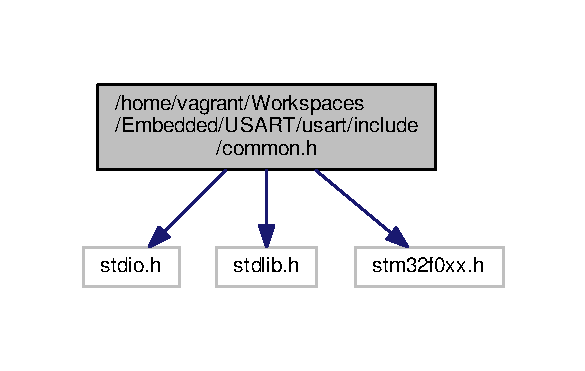
\includegraphics[width=281pt]{common_8h__incl}
\end{center}
\end{figure}
This graph shows which files directly or indirectly include this file\+:
\nopagebreak
\begin{figure}[H]
\begin{center}
\leavevmode
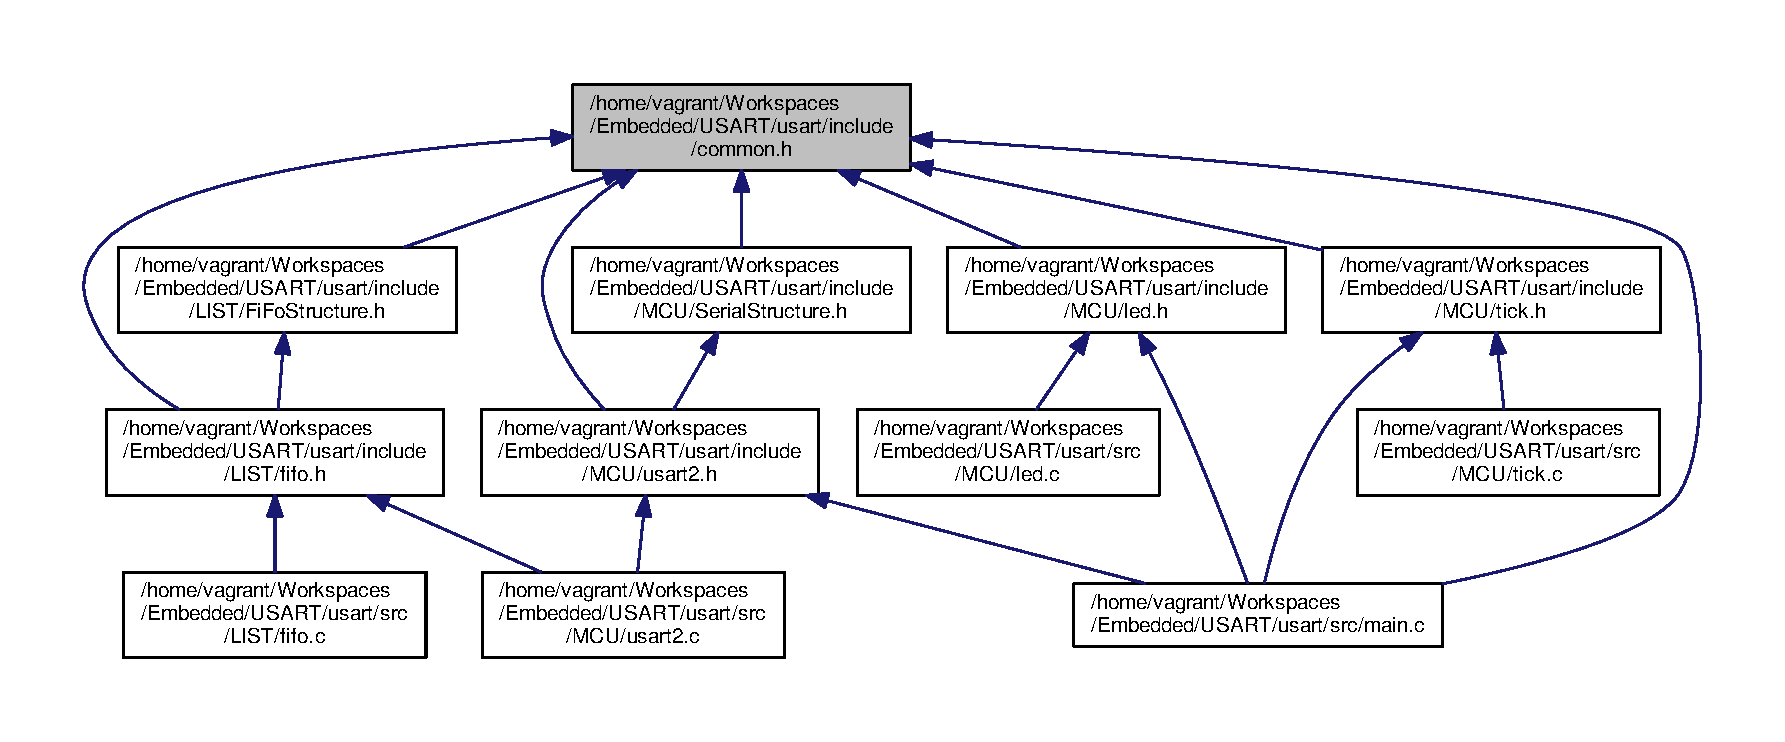
\includegraphics[width=350pt]{common_8h__dep__incl}
\end{center}
\end{figure}
\subsection*{Classes}
\begin{DoxyCompactItemize}
\item 
union \hyperlink{union_data_converter}{Data\+Converter}
\begin{DoxyCompactList}\small\item\em define the union type used to convert between types. \end{DoxyCompactList}\end{DoxyCompactItemize}
\subsection*{Macros}
\begin{DoxyCompactItemize}
\item 
\hypertarget{common_8h_aa8cecfc5c5c054d2875c03e77b7be15d}{\#define \hyperlink{common_8h_aa8cecfc5c5c054d2875c03e77b7be15d}{T\+R\+U\+E}~1}\label{common_8h_aa8cecfc5c5c054d2875c03e77b7be15d}

\begin{DoxyCompactList}\small\item\em Defines the true state. \end{DoxyCompactList}\item 
\hypertarget{common_8h_aa93f0eb578d23995850d61f7d61c55c1}{\#define \hyperlink{common_8h_aa93f0eb578d23995850d61f7d61c55c1}{F\+A\+L\+S\+E}~0}\label{common_8h_aa93f0eb578d23995850d61f7d61c55c1}

\begin{DoxyCompactList}\small\item\em Defines the false state. \end{DoxyCompactList}\item 
\hypertarget{common_8h_a8fe83ac76edc595f6b98cd4a4127aed5}{\#define \hyperlink{common_8h_a8fe83ac76edc595f6b98cd4a4127aed5}{E\+R\+R\+O\+R}~-\/2}\label{common_8h_a8fe83ac76edc595f6b98cd4a4127aed5}

\begin{DoxyCompactList}\small\item\em Defines the error state. \end{DoxyCompactList}\item 
\hypertarget{common_8h_a9109b45a70e8ee7d140b4b4eb097ecea}{\#define \hyperlink{common_8h_a9109b45a70e8ee7d140b4b4eb097ecea}{I\+N\+V\+A\+L\+I\+D\+\_\+\+P\+O\+I\+N\+T\+E\+R\+\_\+\+E\+R\+R\+O\+R}~-\/3}\label{common_8h_a9109b45a70e8ee7d140b4b4eb097ecea}

\begin{DoxyCompactList}\small\item\em Defines the error for invalid pointers. \end{DoxyCompactList}\item 
\#define \hyperlink{common_8h_aa14dc39d52ab121ceb570f1a265385e0}{F\+I\+R\+M\+W\+A\+R\+E\+\_\+\+V\+E\+R\+S\+I\+O\+N}~\char`\"{}00.\+0001\+D\char`\"{}
\begin{DoxyCompactList}\small\item\em Firmware version D = development version of the firmware. Should only be used for testing purposes C = concession version. This version of the firmware is usual custom for a customer. see C\+O\+N\+C\+E\+S\+S\+I\+O\+N\+\_\+\+N\+U\+M\+B\+E\+R P = production version. \end{DoxyCompactList}\item 
\hypertarget{common_8h_a7c770e481dd85c7ffb40e3b3edb0beb5}{\#define \hyperlink{common_8h_a7c770e481dd85c7ffb40e3b3edb0beb5}{H\+A\+R\+D\+W\+A\+R\+E\+\_\+\+V\+E\+R\+S\+I\+O\+N}~\char`\"{}00\char`\"{}}\label{common_8h_a7c770e481dd85c7ffb40e3b3edb0beb5}

\begin{DoxyCompactList}\small\item\em Hardware version. \end{DoxyCompactList}\item 
\hypertarget{common_8h_a4c681fec0533353b247257c82546f7cd}{\#define \hyperlink{common_8h_a4c681fec0533353b247257c82546f7cd}{C\+O\+M\+P\+I\+L\+E\+D\+\_\+\+D\+A\+T\+A\+\_\+\+T\+I\+M\+E}~\char`\"{}\mbox{[}\char`\"{} \+\_\+\+\_\+\+D\+A\+T\+E\+\_\+\+\_\+ \char`\"{} \char`\"{} \+\_\+\+\_\+\+T\+I\+M\+E\+\_\+\+\_\+ \char`\"{}\mbox{]}\char`\"{}}\label{common_8h_a4c681fec0533353b247257c82546f7cd}

\begin{DoxyCompactList}\small\item\em Hardware version. \end{DoxyCompactList}\item 
\hypertarget{common_8h_a5d95e93610ec76137962e82eebebd723}{\#define \hyperlink{common_8h_a5d95e93610ec76137962e82eebebd723}{E\+N\+\_\+\+D\+E\+B\+U\+G\+\_\+\+I\+N\+T\+E\+R\+F\+A\+C\+E}}\label{common_8h_a5d95e93610ec76137962e82eebebd723}

\begin{DoxyCompactList}\small\item\em Enables the debug interface and all debug message associated. \end{DoxyCompactList}\end{DoxyCompactItemize}


\subsection{Detailed Description}
Holds all common code definitions. 

\begin{DoxyAuthor}{Author}
\+: Ronald Sousa () 
\end{DoxyAuthor}


\subsection{Macro Definition Documentation}
\hypertarget{common_8h_aa14dc39d52ab121ceb570f1a265385e0}{\index{common.\+h@{common.\+h}!F\+I\+R\+M\+W\+A\+R\+E\+\_\+\+V\+E\+R\+S\+I\+O\+N@{F\+I\+R\+M\+W\+A\+R\+E\+\_\+\+V\+E\+R\+S\+I\+O\+N}}
\index{F\+I\+R\+M\+W\+A\+R\+E\+\_\+\+V\+E\+R\+S\+I\+O\+N@{F\+I\+R\+M\+W\+A\+R\+E\+\_\+\+V\+E\+R\+S\+I\+O\+N}!common.\+h@{common.\+h}}
\subsubsection[{F\+I\+R\+M\+W\+A\+R\+E\+\_\+\+V\+E\+R\+S\+I\+O\+N}]{\setlength{\rightskip}{0pt plus 5cm}\#define F\+I\+R\+M\+W\+A\+R\+E\+\_\+\+V\+E\+R\+S\+I\+O\+N~\char`\"{}00.\+0001\+D\char`\"{}}}\label{common_8h_aa14dc39d52ab121ceb570f1a265385e0}


Firmware version D = development version of the firmware. Should only be used for testing purposes C = concession version. This version of the firmware is usual custom for a customer. see C\+O\+N\+C\+E\+S\+S\+I\+O\+N\+\_\+\+N\+U\+M\+B\+E\+R P = production version. 

\begin{DoxySeeAlso}{See also}
C\+O\+N\+C\+E\+S\+S\+I\+O\+N\+\_\+\+N\+U\+M\+B\+E\+R 
\end{DoxySeeAlso}

\hypertarget{fifo_8h}{\section{/home/vagrant/\+Workspaces/\+Embedded/\+U\+S\+A\+R\+T/usart/include/\+L\+I\+S\+T/fifo.h File Reference}
\label{fifo_8h}\index{/home/vagrant/\+Workspaces/\+Embedded/\+U\+S\+A\+R\+T/usart/include/\+L\+I\+S\+T/fifo.\+h@{/home/vagrant/\+Workspaces/\+Embedded/\+U\+S\+A\+R\+T/usart/include/\+L\+I\+S\+T/fifo.\+h}}
}


F\+I\+F\+O Library.  


{\ttfamily \#include \char`\"{}../common.\+h\char`\"{}}\\*
{\ttfamily \#include \char`\"{}Fi\+Fo\+Structure.\+h\char`\"{}}\\*
Include dependency graph for fifo.\+h\+:\nopagebreak
\begin{figure}[H]
\begin{center}
\leavevmode
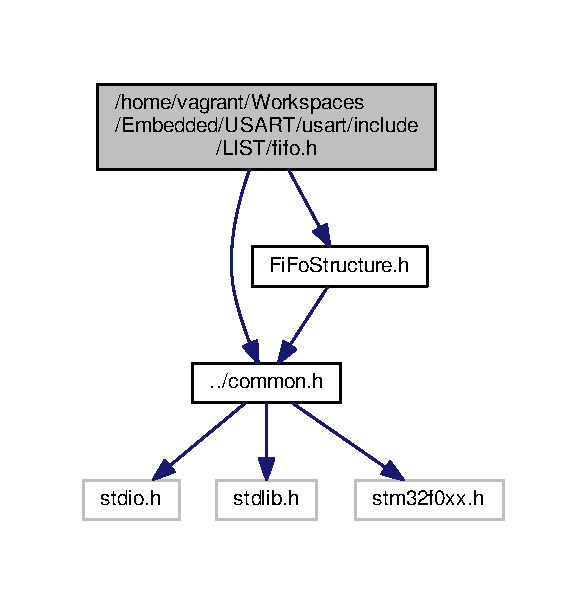
\includegraphics[width=281pt]{fifo_8h__incl}
\end{center}
\end{figure}
This graph shows which files directly or indirectly include this file\+:\nopagebreak
\begin{figure}[H]
\begin{center}
\leavevmode
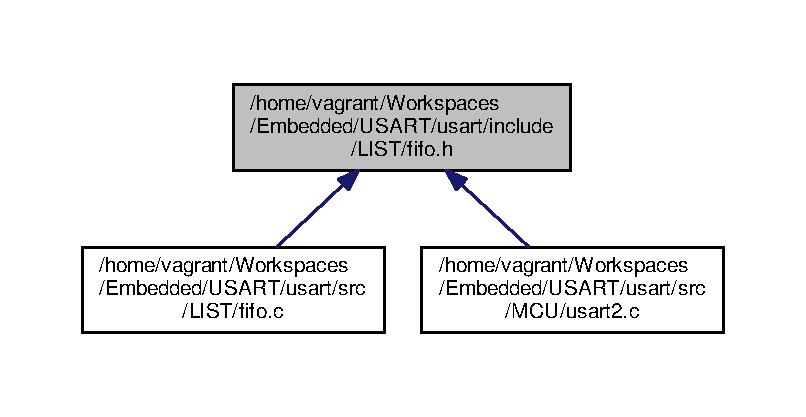
\includegraphics[width=350pt]{fifo_8h__dep__incl}
\end{center}
\end{figure}
\subsection*{Variables}
\begin{DoxyCompactItemize}
\item 
\hyperlink{struct_f_i_f_o_interface}{F\+I\+F\+O\+Interface} \hyperlink{fifo_8h_a01a113408b2025679aeb977f39988432}{F\+I\+F\+O}
\begin{DoxyCompactList}\small\item\em Defines the standard implementation for the F\+I\+F\+O queue. \end{DoxyCompactList}\end{DoxyCompactItemize}


\subsection{Detailed Description}
F\+I\+F\+O Library. 

\begin{DoxyAuthor}{Author}
Steve Mayze 
\end{DoxyAuthor}


\subsection{Variable Documentation}
\hypertarget{fifo_8h_a01a113408b2025679aeb977f39988432}{\index{fifo.\+h@{fifo.\+h}!F\+I\+F\+O@{F\+I\+F\+O}}
\index{F\+I\+F\+O@{F\+I\+F\+O}!fifo.\+h@{fifo.\+h}}
\subsubsection[{F\+I\+F\+O}]{\setlength{\rightskip}{0pt plus 5cm}{\bf F\+I\+F\+O\+Interface} F\+I\+F\+O}}\label{fifo_8h_a01a113408b2025679aeb977f39988432}


Defines the standard implementation for the F\+I\+F\+O queue. 

\begin{DoxySeeAlso}{See also}
\hyperlink{_fi_fo_structure_8h}{Fi\+Fo\+Structure.\+h} 
\end{DoxySeeAlso}

\hypertarget{_fi_fo_structure_8h}{\section{/home/vagrant/\+Workspaces/\+Embedded/\+U\+S\+A\+R\+T/usart/include/\+L\+I\+S\+T/\+Fi\+Fo\+Structure.h File Reference}
\label{_fi_fo_structure_8h}\index{/home/vagrant/\+Workspaces/\+Embedded/\+U\+S\+A\+R\+T/usart/include/\+L\+I\+S\+T/\+Fi\+Fo\+Structure.\+h@{/home/vagrant/\+Workspaces/\+Embedded/\+U\+S\+A\+R\+T/usart/include/\+L\+I\+S\+T/\+Fi\+Fo\+Structure.\+h}}
}


F\+I\+F\+O Library A\+P\+I structure.  


{\ttfamily \#include \char`\"{}../common.\+h\char`\"{}}\\*
Include dependency graph for Fi\+Fo\+Structure.\+h\+:\nopagebreak
\begin{figure}[H]
\begin{center}
\leavevmode
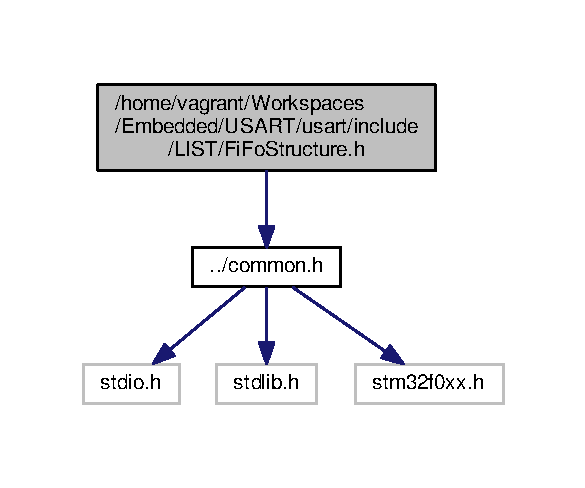
\includegraphics[width=281pt]{_fi_fo_structure_8h__incl}
\end{center}
\end{figure}
This graph shows which files directly or indirectly include this file\+:
\nopagebreak
\begin{figure}[H]
\begin{center}
\leavevmode
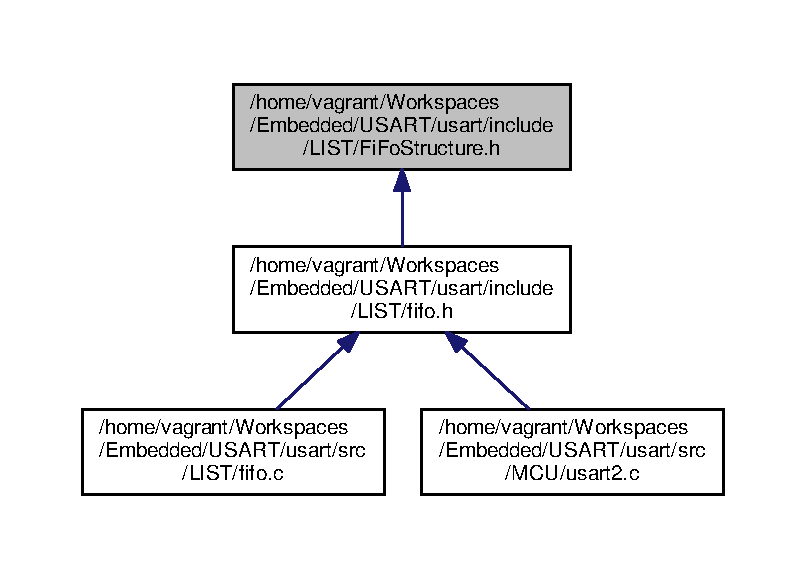
\includegraphics[width=350pt]{_fi_fo_structure_8h__dep__incl}
\end{center}
\end{figure}
\subsection*{Classes}
\begin{DoxyCompactItemize}
\item 
struct \hyperlink{struct_f_i_f_o_queue}{F\+I\+F\+O\+Queue}
\begin{DoxyCompactList}\small\item\em The structure for the F\+I\+F\+O queue as an array of uint8\+\_\+t. \end{DoxyCompactList}\item 
struct \hyperlink{struct_f_i_f_o_interface}{F\+I\+F\+O\+Interface}
\begin{DoxyCompactList}\small\item\em Define the interface for the F\+I\+F\+O list. \end{DoxyCompactList}\end{DoxyCompactItemize}
\subsection*{Macros}
\begin{DoxyCompactItemize}
\item 
\hypertarget{_fi_fo_structure_8h_a8064615b9f07036146ddba2d78ab43ac}{\#define \hyperlink{_fi_fo_structure_8h_a8064615b9f07036146ddba2d78ab43ac}{M\+A\+X\+Q\+U\+E\+U\+E\+S\+I\+Z\+E}~256}\label{_fi_fo_structure_8h_a8064615b9f07036146ddba2d78ab43ac}

\begin{DoxyCompactList}\small\item\em defines the F\+I\+F\+O buffer maximum size \end{DoxyCompactList}\end{DoxyCompactItemize}


\subsection{Detailed Description}
F\+I\+F\+O Library A\+P\+I structure. 

\begin{DoxyAuthor}{Author}
Steve Mayze 
\end{DoxyAuthor}

\hypertarget{led_8h}{\section{/home/vagrant/\+Workspaces/\+Embedded/\+U\+S\+A\+R\+T/usart/include/\+M\+C\+U/led.h File Reference}
\label{led_8h}\index{/home/vagrant/\+Workspaces/\+Embedded/\+U\+S\+A\+R\+T/usart/include/\+M\+C\+U/led.\+h@{/home/vagrant/\+Workspaces/\+Embedded/\+U\+S\+A\+R\+T/usart/include/\+M\+C\+U/led.\+h}}
}
{\ttfamily \#include \char`\"{}common.\+h\char`\"{}}\\*
Include dependency graph for led.\+h\+:\nopagebreak
\begin{figure}[H]
\begin{center}
\leavevmode
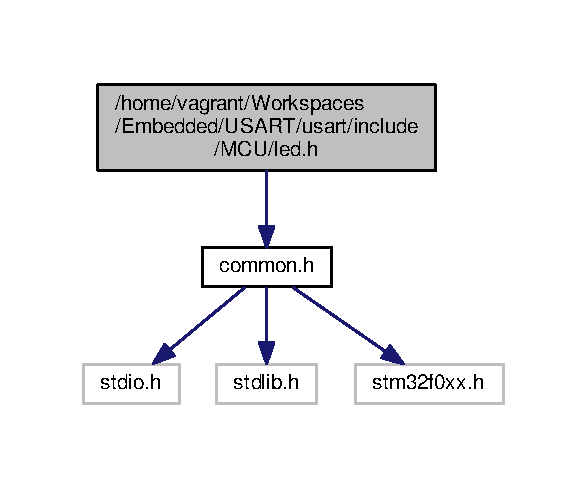
\includegraphics[width=281pt]{led_8h__incl}
\end{center}
\end{figure}
This graph shows which files directly or indirectly include this file\+:\nopagebreak
\begin{figure}[H]
\begin{center}
\leavevmode
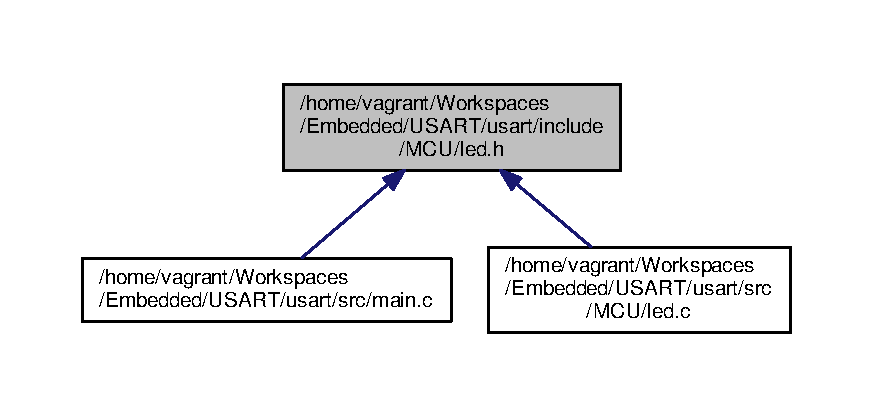
\includegraphics[width=350pt]{led_8h__dep__incl}
\end{center}
\end{figure}
\subsection*{Functions}
\begin{DoxyCompactItemize}
\item 
\hypertarget{led_8h_af1aee968a5ceeb7915921aa6d78aca23}{void \hyperlink{led_8h_af1aee968a5ceeb7915921aa6d78aca23}{Led\+\_\+\+Init} (void)}\label{led_8h_af1aee968a5ceeb7915921aa6d78aca23}

\begin{DoxyCompactList}\small\item\em Setup the L\+E\+D I\+O. \end{DoxyCompactList}\item 
\hypertarget{led_8h_a39675df62ae72fa5af35fc7ec2e8c950}{void \hyperlink{led_8h_a39675df62ae72fa5af35fc7ec2e8c950}{Led\+\_\+\+On} (void)}\label{led_8h_a39675df62ae72fa5af35fc7ec2e8c950}

\begin{DoxyCompactList}\small\item\em Turns on the L\+E\+D. \end{DoxyCompactList}\item 
\hypertarget{led_8h_a274dbef77287444be852fe96969b3c55}{void \hyperlink{led_8h_a274dbef77287444be852fe96969b3c55}{Led\+\_\+\+Off} (void)}\label{led_8h_a274dbef77287444be852fe96969b3c55}

\begin{DoxyCompactList}\small\item\em Turns off the L\+E\+D. \end{DoxyCompactList}\item 
\hypertarget{led_8h_a5ebbd778fb3444fbfbded2130e08b33d}{void \hyperlink{led_8h_a5ebbd778fb3444fbfbded2130e08b33d}{Led\+\_\+\+Toggle} (void)}\label{led_8h_a5ebbd778fb3444fbfbded2130e08b33d}

\begin{DoxyCompactList}\small\item\em Toggle the L\+E\+D state. \end{DoxyCompactList}\end{DoxyCompactItemize}


\subsection{Detailed Description}
Author\+: Ronald Sousa () 
\hypertarget{_serial_structure_8h}{\section{/home/vagrant/\+Workspaces/\+Embedded/\+U\+S\+A\+R\+T/usart/include/\+M\+C\+U/\+Serial\+Structure.h File Reference}
\label{_serial_structure_8h}\index{/home/vagrant/\+Workspaces/\+Embedded/\+U\+S\+A\+R\+T/usart/include/\+M\+C\+U/\+Serial\+Structure.\+h@{/home/vagrant/\+Workspaces/\+Embedded/\+U\+S\+A\+R\+T/usart/include/\+M\+C\+U/\+Serial\+Structure.\+h}}
}


define the serial interface layer structure  


{\ttfamily \#include \char`\"{}../common.\+h\char`\"{}}\\*
Include dependency graph for Serial\+Structure.\+h\+:\nopagebreak
\begin{figure}[H]
\begin{center}
\leavevmode
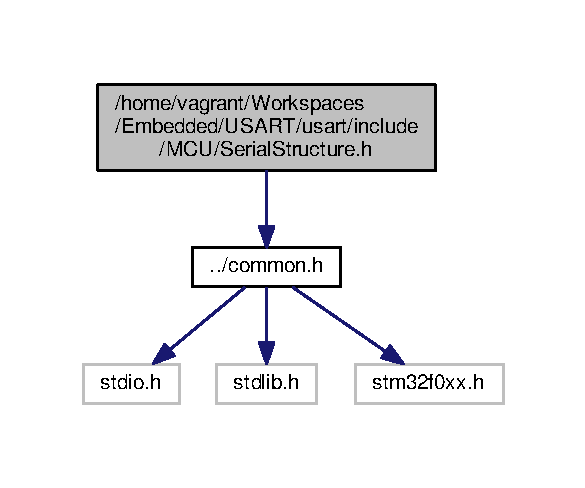
\includegraphics[width=281pt]{_serial_structure_8h__incl}
\end{center}
\end{figure}
This graph shows which files directly or indirectly include this file\+:\nopagebreak
\begin{figure}[H]
\begin{center}
\leavevmode
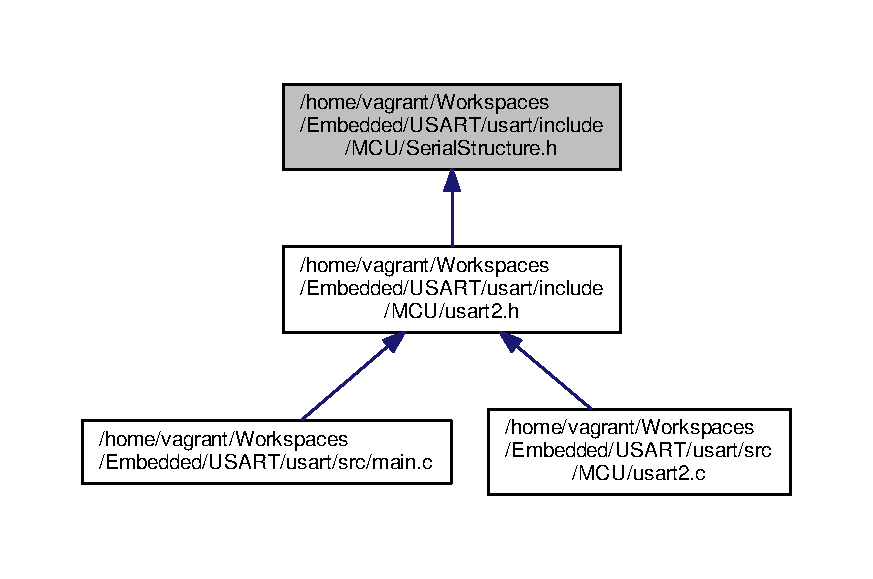
\includegraphics[width=350pt]{_serial_structure_8h__dep__incl}
\end{center}
\end{figure}
\subsection*{Classes}
\begin{DoxyCompactItemize}
\item 
struct \hyperlink{struct_serial_interface}{Serial\+Interface}
\begin{DoxyCompactList}\small\item\em define the standard serial interface \end{DoxyCompactList}\end{DoxyCompactItemize}


\subsection{Detailed Description}
define the serial interface layer structure 

\begin{DoxyAuthor}{Author}
Ronald Sousa  www.\+Hash\+Define\+Electronics.\+com  Hash Define Electronics Ltd 
\end{DoxyAuthor}

\hypertarget{tick_8h}{\section{/home/vagrant/\+Workspaces/\+Embedded/\+U\+S\+A\+R\+T/usart/include/\+M\+C\+U/tick.h File Reference}
\label{tick_8h}\index{/home/vagrant/\+Workspaces/\+Embedded/\+U\+S\+A\+R\+T/usart/include/\+M\+C\+U/tick.\+h@{/home/vagrant/\+Workspaces/\+Embedded/\+U\+S\+A\+R\+T/usart/include/\+M\+C\+U/tick.\+h}}
}
{\ttfamily \#include \char`\"{}common.\+h\char`\"{}}\\*
Include dependency graph for tick.\+h\+:\nopagebreak
\begin{figure}[H]
\begin{center}
\leavevmode
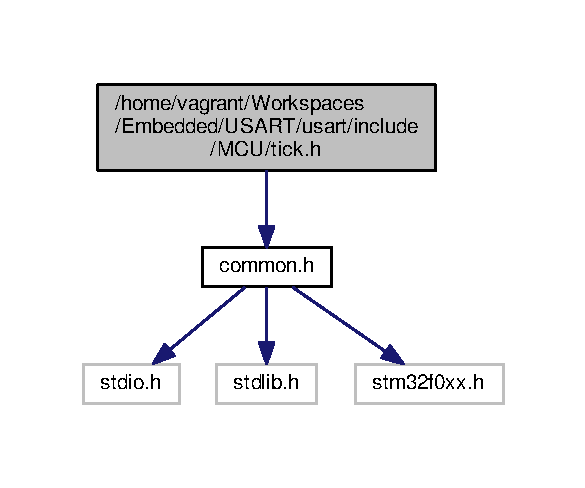
\includegraphics[width=281pt]{tick_8h__incl}
\end{center}
\end{figure}
This graph shows which files directly or indirectly include this file\+:\nopagebreak
\begin{figure}[H]
\begin{center}
\leavevmode
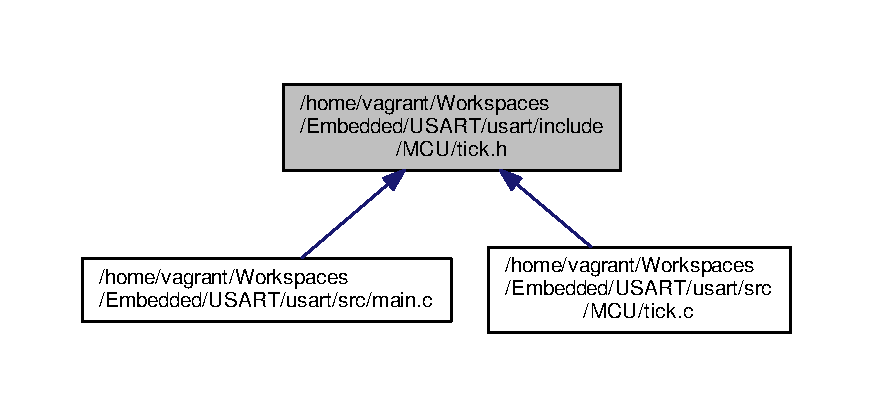
\includegraphics[width=350pt]{tick_8h__dep__incl}
\end{center}
\end{figure}
\subsection*{Classes}
\begin{DoxyCompactItemize}
\item 
struct \hyperlink{struct_tick_type}{Tick\+Type}
\begin{DoxyCompactList}\small\item\em defines a non-\/blocking delay data type. \end{DoxyCompactList}\end{DoxyCompactItemize}
\subsection*{Functions}
\begin{DoxyCompactItemize}
\item 
\hypertarget{tick_8h_ade660961e7af4755750dd6ff81535e68}{void \hyperlink{tick_8h_ade660961e7af4755750dd6ff81535e68}{Tick\+\_\+init} (void)}\label{tick_8h_ade660961e7af4755750dd6ff81535e68}

\begin{DoxyCompactList}\small\item\em setup the A\+R\+M M0 tick counter to trigger every 1ms \end{DoxyCompactList}\item 
uint32\+\_\+t \hyperlink{tick_8h_a5018c28a90fe9864e870a712c8e2b571}{Tick\+\_\+\+Get\+Ms} (void)
\begin{DoxyCompactList}\small\item\em return the number of mili-\/seconds since power up. \end{DoxyCompactList}\item 
int\+\_\+fast8\+\_\+t \hyperlink{tick_8h_a700a086c5fb6a2a2491026af0fda77a8}{Tick\+\_\+\+Delay\+Ms\+\_\+\+Non\+Blocking} (uint\+\_\+fast8\+\_\+t reset, \hyperlink{struct_tick_type}{Tick\+Type} $\ast$config)
\begin{DoxyCompactList}\small\item\em Non-\/blocking delay in ms. \end{DoxyCompactList}\item 
void \hyperlink{tick_8h_a01864fcfa99d364250b9e3e10390ff93}{Tick\+\_\+\+Delay\+Ms} (uint32\+\_\+t delay\+Ms)
\begin{DoxyCompactList}\small\item\em this is a blocking delay. \end{DoxyCompactList}\end{DoxyCompactItemize}


\subsection{Detailed Description}
Author\+: Ronald Sousa () 

\subsection{Function Documentation}
\hypertarget{tick_8h_a01864fcfa99d364250b9e3e10390ff93}{\index{tick.\+h@{tick.\+h}!Tick\+\_\+\+Delay\+Ms@{Tick\+\_\+\+Delay\+Ms}}
\index{Tick\+\_\+\+Delay\+Ms@{Tick\+\_\+\+Delay\+Ms}!tick.\+h@{tick.\+h}}
\subsubsection[{Tick\+\_\+\+Delay\+Ms}]{\setlength{\rightskip}{0pt plus 5cm}void Tick\+\_\+\+Delay\+Ms (
\begin{DoxyParamCaption}
\item[{uint32\+\_\+t}]{delay\+Ms}
\end{DoxyParamCaption}
)}}\label{tick_8h_a01864fcfa99d364250b9e3e10390ff93}


this is a blocking delay. 


\begin{DoxyCode}
\textcolor{preprocessor}{ #include "\hyperlink{common_8h}{common.h}"}
\textcolor{preprocessor}{ #include "\hyperlink{led_8h}{MCU/led.h}"}
\textcolor{preprocessor}{ #include "\hyperlink{tick_8h}{MCU/tick.h}"}

 \textcolor{keywordtype}{void} \hyperlink{main_8c_a6288eba0f8e8ad3ab1544ad731eb7667}{main}(\textcolor{keywordtype}{void}) \{

     \hyperlink{led_8c_af1aee968a5ceeb7915921aa6d78aca23}{Led\_Init}();
     \hyperlink{tick_8c_ade660961e7af4755750dd6ff81535e68}{Tick\_init}();

     \textcolor{keywordflow}{for}( ;;) \{
       \hyperlink{tick_8c_a01864fcfa99d364250b9e3e10390ff93}{Tick\_DelayMs}(1000); \textcolor{comment}{// delay 1s;}
       \hyperlink{led_8c_a5ebbd778fb3444fbfbded2130e08b33d}{Led\_Toggle}();
     \}
\}
\end{DoxyCode}



\begin{DoxyParams}{Parameters}
{\em delay\+Ms} & how long to delay for. \\
\hline
\end{DoxyParams}


Here is the caller graph for this function\+:
\nopagebreak
\begin{figure}[H]
\begin{center}
\leavevmode
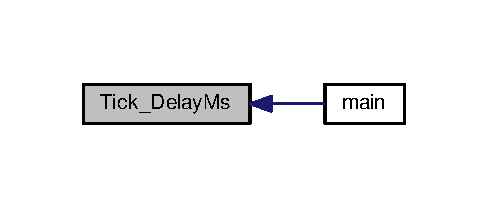
\includegraphics[width=234pt]{tick_8h_a01864fcfa99d364250b9e3e10390ff93_icgraph}
\end{center}
\end{figure}


\hypertarget{tick_8h_a700a086c5fb6a2a2491026af0fda77a8}{\index{tick.\+h@{tick.\+h}!Tick\+\_\+\+Delay\+Ms\+\_\+\+Non\+Blocking@{Tick\+\_\+\+Delay\+Ms\+\_\+\+Non\+Blocking}}
\index{Tick\+\_\+\+Delay\+Ms\+\_\+\+Non\+Blocking@{Tick\+\_\+\+Delay\+Ms\+\_\+\+Non\+Blocking}!tick.\+h@{tick.\+h}}
\subsubsection[{Tick\+\_\+\+Delay\+Ms\+\_\+\+Non\+Blocking}]{\setlength{\rightskip}{0pt plus 5cm}int\+\_\+fast8\+\_\+t Tick\+\_\+\+Delay\+Ms\+\_\+\+Non\+Blocking (
\begin{DoxyParamCaption}
\item[{uint\+\_\+fast8\+\_\+t}]{reset, }
\item[{{\bf Tick\+Type} $\ast$}]{config}
\end{DoxyParamCaption}
)}}\label{tick_8h_a700a086c5fb6a2a2491026af0fda77a8}


Non-\/blocking delay in ms. 


\begin{DoxyCode}
\textcolor{preprocessor}{ #include "\hyperlink{common_8h}{common.h}"}
\textcolor{preprocessor}{ #include "\hyperlink{led_8h}{MCU/led.h}"}
\textcolor{preprocessor}{ #include "\hyperlink{tick_8h}{MCU/tick.h}"}

 \textcolor{keywordtype}{void} \hyperlink{main_8c_a6288eba0f8e8ad3ab1544ad731eb7667}{main}(\textcolor{keywordtype}{void}) \{
     \hyperlink{struct_tick_type}{TickType} Delay;
     Delay.\hyperlink{struct_tick_type_ae24ecd63a2b008c5c9a6864cbb3b30a7}{DelayMs} = 1000; \textcolor{comment}{//set to 1s}

     \hyperlink{led_8c_af1aee968a5ceeb7915921aa6d78aca23}{Led\_Init}();
     \hyperlink{tick_8c_ade660961e7af4755750dd6ff81535e68}{Tick\_init}();

     \textcolor{comment}{// reset the counter}
     \hyperlink{tick_8c_a700a086c5fb6a2a2491026af0fda77a8}{Tick\_DelayMs\_NonBlocking}(\hyperlink{common_8h_aa8cecfc5c5c054d2875c03e77b7be15d}{TRUE}, &Delay);

     \textcolor{keywordflow}{for}( ;;) \{

         \textcolor{keywordflow}{if}(\hyperlink{tick_8c_a700a086c5fb6a2a2491026af0fda77a8}{Tick\_DelayMs\_NonBlocking}(\hyperlink{common_8h_aa8cecfc5c5c054d2875c03e77b7be15d}{TRUE}, &Delay)) \{
             \textcolor{comment}{// Delay has been reached}

             \hyperlink{tick_8c_a700a086c5fb6a2a2491026af0fda77a8}{Tick\_DelayMs\_NonBlocking}(\hyperlink{common_8h_aa8cecfc5c5c054d2875c03e77b7be15d}{TRUE}, &Delay);
             \hyperlink{led_8c_a5ebbd778fb3444fbfbded2130e08b33d}{Led\_Toggle}();
             \}
         \textcolor{keywordflow}{else} \{
             \textcolor{comment}{// User code when the code delay hasn't passed}
             \}

     \}
\}
\end{DoxyCode}



\begin{DoxyParams}{Parameters}
{\em reset} & true = reset timer start value/ false = Check if time has lapsed \\
\hline
{\em config} & delay setting\\
\hline
\end{DoxyParams}
\begin{DoxyReturn}{Returns}
1 = the desire delay has been reached. 0 = not reached the desire delay time. -\/1 = config point is null 
\end{DoxyReturn}


Here is the call graph for this function\+:\nopagebreak
\begin{figure}[H]
\begin{center}
\leavevmode
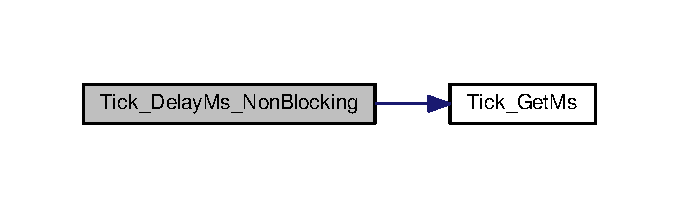
\includegraphics[width=326pt]{tick_8h_a700a086c5fb6a2a2491026af0fda77a8_cgraph}
\end{center}
\end{figure}


\hypertarget{tick_8h_a5018c28a90fe9864e870a712c8e2b571}{\index{tick.\+h@{tick.\+h}!Tick\+\_\+\+Get\+Ms@{Tick\+\_\+\+Get\+Ms}}
\index{Tick\+\_\+\+Get\+Ms@{Tick\+\_\+\+Get\+Ms}!tick.\+h@{tick.\+h}}
\subsubsection[{Tick\+\_\+\+Get\+Ms}]{\setlength{\rightskip}{0pt plus 5cm}uint32\+\_\+t Tick\+\_\+\+Get\+Ms (
\begin{DoxyParamCaption}
\item[{void}]{}
\end{DoxyParamCaption}
)}}\label{tick_8h_a5018c28a90fe9864e870a712c8e2b571}


return the number of mili-\/seconds since power up. 

\begin{DoxyReturn}{Returns}
number of mili-\/seconds.
\end{DoxyReturn}
\begin{DoxyNote}{Note}
the tick counter is expected to overflow and therefore code using the tick value should take this into account. 
\end{DoxyNote}


Here is the caller graph for this function\+:\nopagebreak
\begin{figure}[H]
\begin{center}
\leavevmode
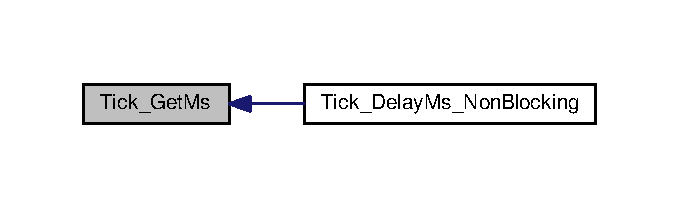
\includegraphics[width=326pt]{tick_8h_a5018c28a90fe9864e870a712c8e2b571_icgraph}
\end{center}
\end{figure}



\hypertarget{usart2_8h}{\section{/home/vagrant/\+Workspaces/\+Embedded/\+U\+S\+A\+R\+T/usart/include/\+M\+C\+U/usart2.h File Reference}
\label{usart2_8h}\index{/home/vagrant/\+Workspaces/\+Embedded/\+U\+S\+A\+R\+T/usart/include/\+M\+C\+U/usart2.\+h@{/home/vagrant/\+Workspaces/\+Embedded/\+U\+S\+A\+R\+T/usart/include/\+M\+C\+U/usart2.\+h}}
}
{\ttfamily \#include \char`\"{}common.\+h\char`\"{}}\\*
{\ttfamily \#include \char`\"{}M\+C\+U/\+Serial\+Structure.\+h\char`\"{}}\\*
Include dependency graph for usart2.\+h\+:\nopagebreak
\begin{figure}[H]
\begin{center}
\leavevmode
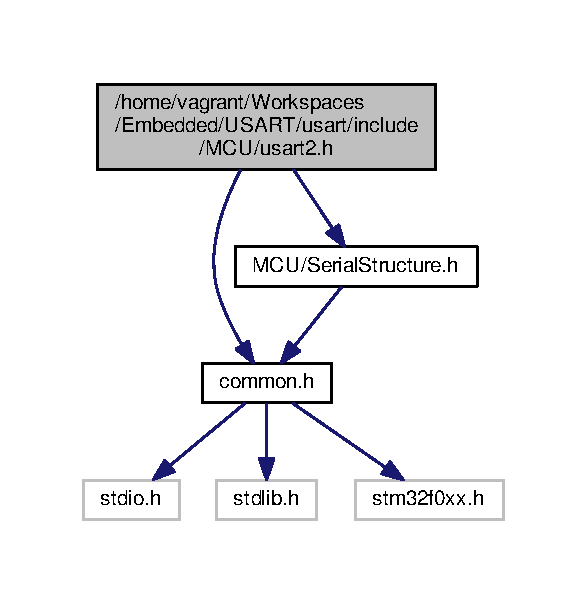
\includegraphics[width=281pt]{usart2_8h__incl}
\end{center}
\end{figure}
This graph shows which files directly or indirectly include this file\+:\nopagebreak
\begin{figure}[H]
\begin{center}
\leavevmode
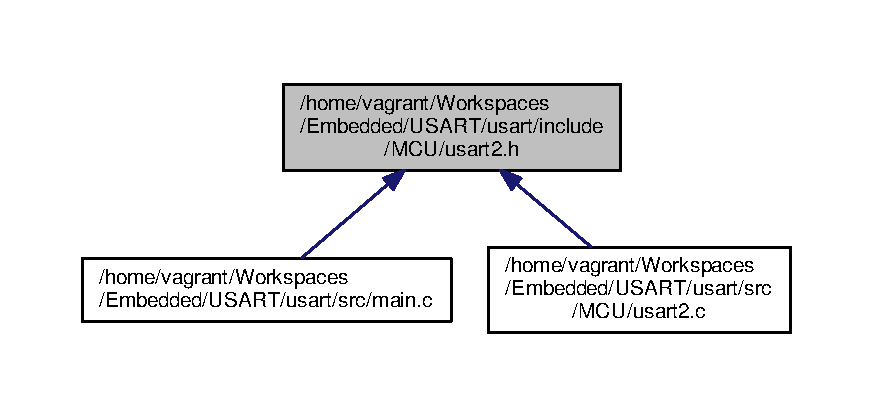
\includegraphics[width=350pt]{usart2_8h__dep__incl}
\end{center}
\end{figure}
\subsection*{Variables}
\begin{DoxyCompactItemize}
\item 
\hyperlink{struct_serial_interface}{Serial\+Interface} \hyperlink{usart2_8h_a0ad9cd4fbffc7497abd537641dcc99af}{Serial\+Port2}
\begin{DoxyCompactList}\small\item\em Defines the standard serial functions for usart 2. \end{DoxyCompactList}\end{DoxyCompactItemize}


\subsection{Detailed Description}
\begin{DoxyAuthor}{Author}
\+: Ronald Sousa () 
\end{DoxyAuthor}


\subsection{Variable Documentation}
\hypertarget{usart2_8h_a0ad9cd4fbffc7497abd537641dcc99af}{\index{usart2.\+h@{usart2.\+h}!Serial\+Port2@{Serial\+Port2}}
\index{Serial\+Port2@{Serial\+Port2}!usart2.\+h@{usart2.\+h}}
\subsubsection[{Serial\+Port2}]{\setlength{\rightskip}{0pt plus 5cm}{\bf Serial\+Interface} Serial\+Port2}}\label{usart2_8h_a0ad9cd4fbffc7497abd537641dcc99af}


Defines the standard serial functions for usart 2. 

\begin{DoxySeeAlso}{See also}
\hyperlink{struct_serial_interface}{Serial\+Interface} 
\end{DoxySeeAlso}

\hypertarget{fifo_8c}{\section{/home/vagrant/\+Workspaces/\+Embedded/\+U\+S\+A\+R\+T/usart/src/\+L\+I\+S\+T/fifo.c File Reference}
\label{fifo_8c}\index{/home/vagrant/\+Workspaces/\+Embedded/\+U\+S\+A\+R\+T/usart/src/\+L\+I\+S\+T/fifo.\+c@{/home/vagrant/\+Workspaces/\+Embedded/\+U\+S\+A\+R\+T/usart/src/\+L\+I\+S\+T/fifo.\+c}}
}


F\+I\+F\+O Library.  


{\ttfamily \#include \char`\"{}L\+I\+S\+T/fifo.\+h\char`\"{}}\\*
Include dependency graph for fifo.\+c\+:\nopagebreak
\begin{figure}[H]
\begin{center}
\leavevmode
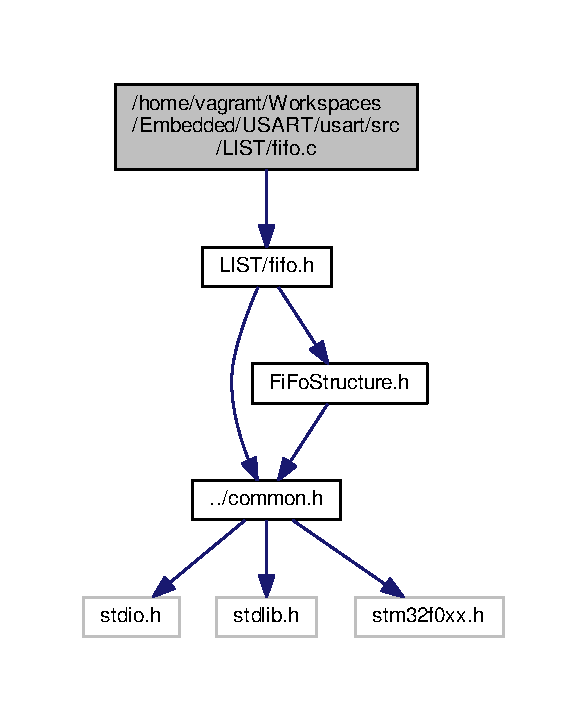
\includegraphics[width=281pt]{fifo_8c__incl}
\end{center}
\end{figure}
\subsection*{Variables}
\begin{DoxyCompactItemize}
\item 
\hyperlink{struct_f_i_f_o_interface}{F\+I\+F\+O\+Interface} \hyperlink{fifo_8c_a01a113408b2025679aeb977f39988432}{F\+I\+F\+O}
\begin{DoxyCompactList}\small\item\em Defines the standard implementation for the F\+I\+F\+O queue. \end{DoxyCompactList}\end{DoxyCompactItemize}


\subsection{Detailed Description}
F\+I\+F\+O Library. 

\begin{DoxyAuthor}{Author}
Steve Mayze
\end{DoxyAuthor}

\begin{DoxyImage}
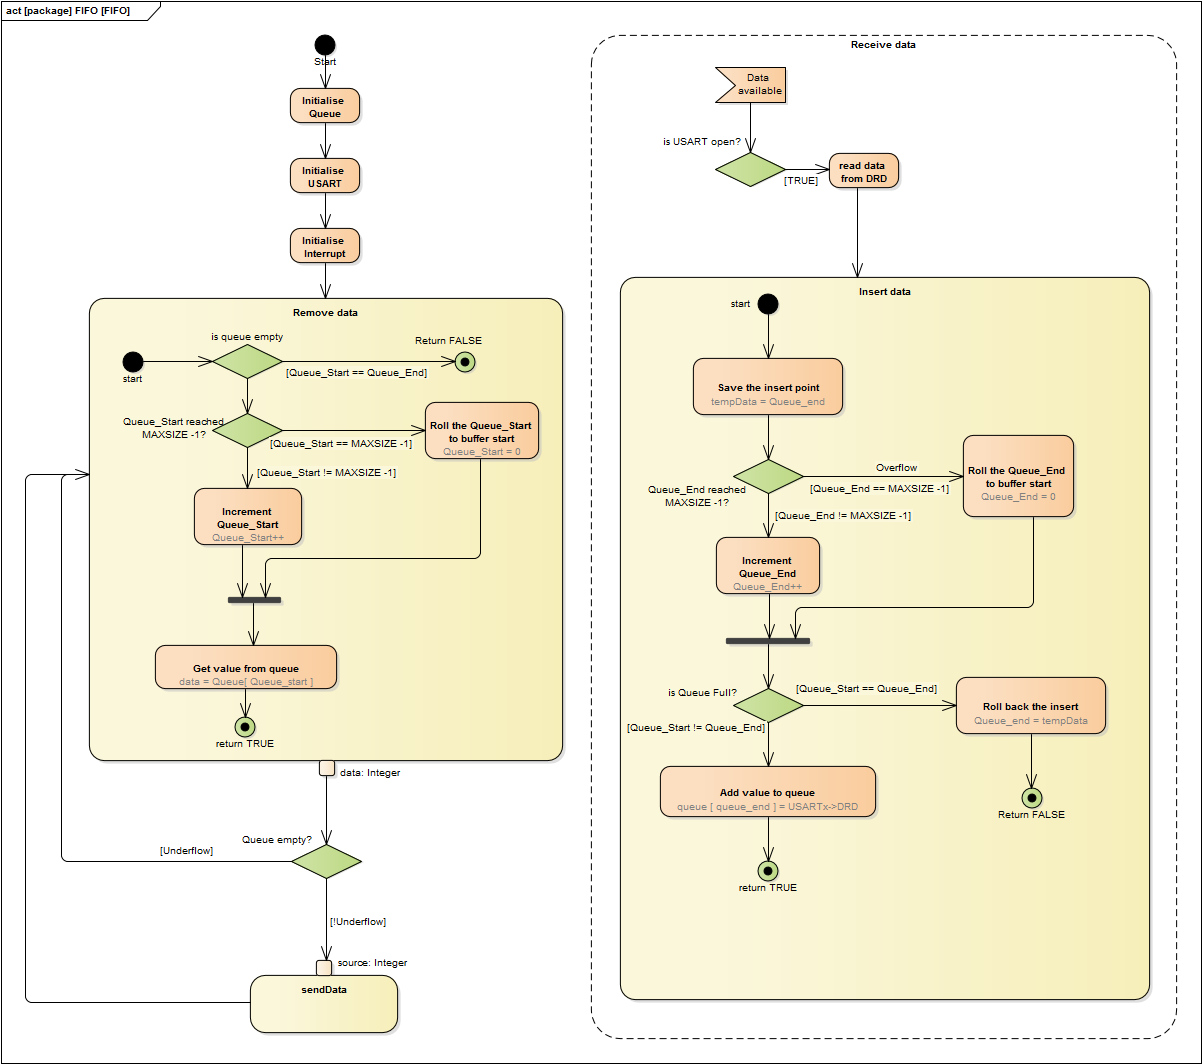
\includegraphics[width=15cm]{FIFO.png}
\caption{F\+I\+F\+O A\+P\+I Activity diagram}
\end{DoxyImage}
 

\subsection{Variable Documentation}
\hypertarget{fifo_8c_a01a113408b2025679aeb977f39988432}{\index{fifo.\+c@{fifo.\+c}!F\+I\+F\+O@{F\+I\+F\+O}}
\index{F\+I\+F\+O@{F\+I\+F\+O}!fifo.\+c@{fifo.\+c}}
\subsubsection[{F\+I\+F\+O}]{\setlength{\rightskip}{0pt plus 5cm}{\bf F\+I\+F\+O\+Interface} F\+I\+F\+O}}\label{fifo_8c_a01a113408b2025679aeb977f39988432}
{\bfseries Initial value\+:}
\begin{DoxyCode}
= \{
        Initialize,
        Insert,
        Remove
\}
\end{DoxyCode}


Defines the standard implementation for the F\+I\+F\+O queue. 

\begin{DoxySeeAlso}{See also}
\hyperlink{_fi_fo_structure_8h}{Fi\+Fo\+Structure.\+h} 
\end{DoxySeeAlso}

\hypertarget{main_8c}{\section{/home/vagrant/\+Workspaces/\+Embedded/\+U\+S\+A\+R\+T/usart/src/main.c File Reference}
\label{main_8c}\index{/home/vagrant/\+Workspaces/\+Embedded/\+U\+S\+A\+R\+T/usart/src/main.\+c@{/home/vagrant/\+Workspaces/\+Embedded/\+U\+S\+A\+R\+T/usart/src/main.\+c}}
}


This is the main program code.  


{\ttfamily \#include \char`\"{}common.\+h\char`\"{}}\\*
{\ttfamily \#include \char`\"{}M\+C\+U/led.\+h\char`\"{}}\\*
{\ttfamily \#include \char`\"{}M\+C\+U/usart2.\+h\char`\"{}}\\*
{\ttfamily \#include \char`\"{}M\+C\+U/tick.\+h\char`\"{}}\\*
{\ttfamily \#include \char`\"{}L\+I\+S\+T/fifo.\+h\char`\"{}}\\*
Include dependency graph for main.\+c\+:\nopagebreak
\begin{figure}[H]
\begin{center}
\leavevmode
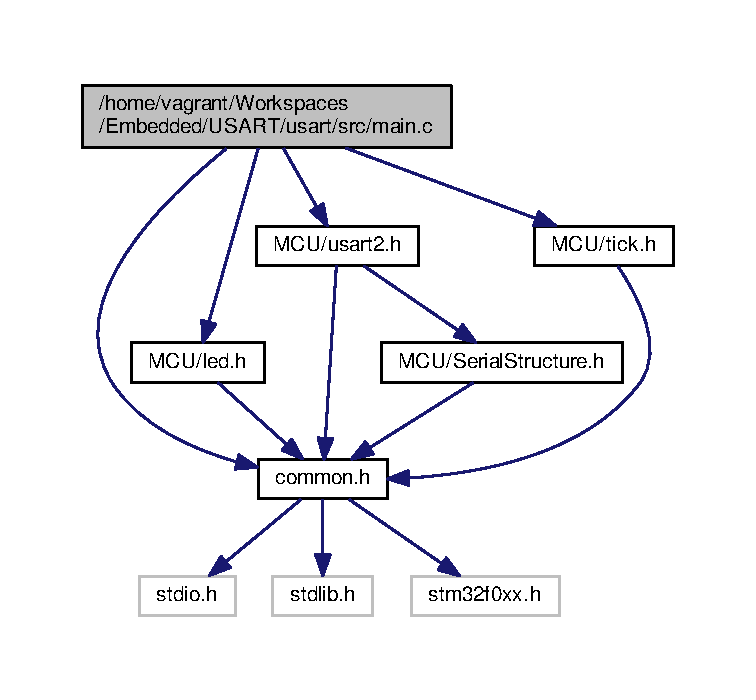
\includegraphics[width=350pt]{main_8c__incl}
\end{center}
\end{figure}
\subsection*{Functions}
\begin{DoxyCompactItemize}
\item 
\hypertarget{main_8c_a6288eba0f8e8ad3ab1544ad731eb7667}{void \hyperlink{main_8c_a6288eba0f8e8ad3ab1544ad731eb7667}{main} (void)}\label{main_8c_a6288eba0f8e8ad3ab1544ad731eb7667}

\begin{DoxyCompactList}\small\item\em the first user code function to be called after the A\+R\+M M0 has initial. \end{DoxyCompactList}\end{DoxyCompactItemize}


\subsection{Detailed Description}
This is the main program code. 

\begin{DoxyAuthor}{Author}
\+: Ronald Sousa (Opticalworm) 
\end{DoxyAuthor}

\hypertarget{led_8c}{\section{/home/vagrant/\+Workspaces/\+Embedded/\+U\+S\+A\+R\+T/usart/src/\+M\+C\+U/led.c File Reference}
\label{led_8c}\index{/home/vagrant/\+Workspaces/\+Embedded/\+U\+S\+A\+R\+T/usart/src/\+M\+C\+U/led.\+c@{/home/vagrant/\+Workspaces/\+Embedded/\+U\+S\+A\+R\+T/usart/src/\+M\+C\+U/led.\+c}}
}


this is the L\+E\+D hardware interface layer.  


{\ttfamily \#include \char`\"{}M\+C\+U/led.\+h\char`\"{}}\\*
Include dependency graph for led.\+c\+:\nopagebreak
\begin{figure}[H]
\begin{center}
\leavevmode
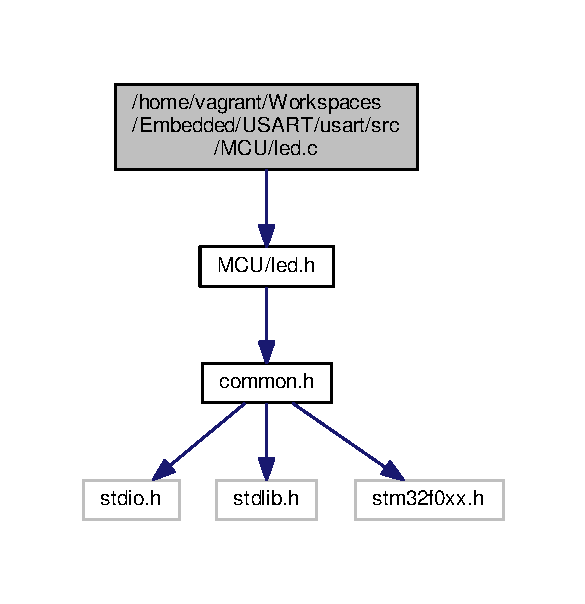
\includegraphics[width=281pt]{led_8c__incl}
\end{center}
\end{figure}
\subsection*{Macros}
\begin{DoxyCompactItemize}
\item 
\hypertarget{led_8c_ab4553be4db9860d940f81d7447173b2f}{\#define \hyperlink{led_8c_ab4553be4db9860d940f81d7447173b2f}{L\+E\+D\+\_\+\+P\+I\+N}~5}\label{led_8c_ab4553be4db9860d940f81d7447173b2f}

\begin{DoxyCompactList}\small\item\em defines the L\+E\+D pin number \end{DoxyCompactList}\end{DoxyCompactItemize}
\subsection*{Functions}
\begin{DoxyCompactItemize}
\item 
\hypertarget{led_8c_a39675df62ae72fa5af35fc7ec2e8c950}{void \hyperlink{led_8c_a39675df62ae72fa5af35fc7ec2e8c950}{Led\+\_\+\+On} (void)}\label{led_8c_a39675df62ae72fa5af35fc7ec2e8c950}

\begin{DoxyCompactList}\small\item\em Turns on the L\+E\+D. \end{DoxyCompactList}\item 
\hypertarget{led_8c_a274dbef77287444be852fe96969b3c55}{void \hyperlink{led_8c_a274dbef77287444be852fe96969b3c55}{Led\+\_\+\+Off} (void)}\label{led_8c_a274dbef77287444be852fe96969b3c55}

\begin{DoxyCompactList}\small\item\em Turns off the L\+E\+D. \end{DoxyCompactList}\item 
\hypertarget{led_8c_a5ebbd778fb3444fbfbded2130e08b33d}{void \hyperlink{led_8c_a5ebbd778fb3444fbfbded2130e08b33d}{Led\+\_\+\+Toggle} (void)}\label{led_8c_a5ebbd778fb3444fbfbded2130e08b33d}

\begin{DoxyCompactList}\small\item\em Toggle the L\+E\+D state. \end{DoxyCompactList}\item 
\hypertarget{led_8c_af1aee968a5ceeb7915921aa6d78aca23}{void \hyperlink{led_8c_af1aee968a5ceeb7915921aa6d78aca23}{Led\+\_\+\+Init} (void)}\label{led_8c_af1aee968a5ceeb7915921aa6d78aca23}

\begin{DoxyCompactList}\small\item\em Setup the L\+E\+D I\+O. \end{DoxyCompactList}\end{DoxyCompactItemize}


\subsection{Detailed Description}
this is the L\+E\+D hardware interface layer. 

\begin{DoxyAuthor}{Author}
\+: Ronald Sousa () 
\end{DoxyAuthor}

\hypertarget{tick_8c}{\section{/home/vagrant/\+Workspaces/\+Embedded/\+U\+S\+A\+R\+T/usart/src/\+M\+C\+U/tick.c File Reference}
\label{tick_8c}\index{/home/vagrant/\+Workspaces/\+Embedded/\+U\+S\+A\+R\+T/usart/src/\+M\+C\+U/tick.\+c@{/home/vagrant/\+Workspaces/\+Embedded/\+U\+S\+A\+R\+T/usart/src/\+M\+C\+U/tick.\+c}}
}


implements mili-\/second tick counter.  


{\ttfamily \#include \char`\"{}M\+C\+U/tick.\+h\char`\"{}}\\*
Include dependency graph for tick.\+c\+:\nopagebreak
\begin{figure}[H]
\begin{center}
\leavevmode
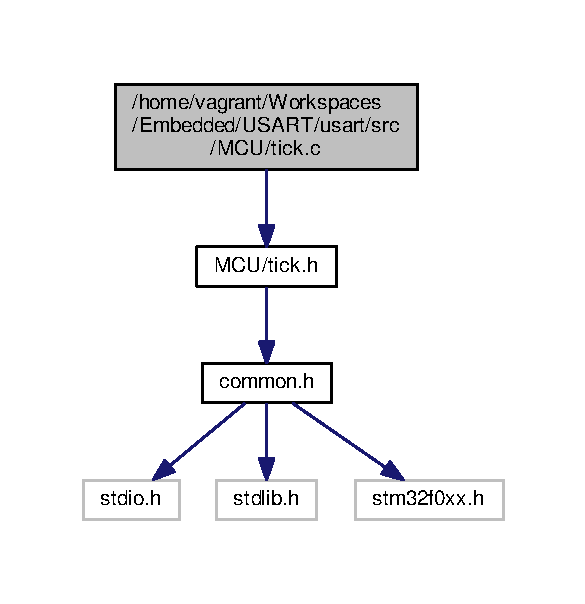
\includegraphics[width=281pt]{tick_8c__incl}
\end{center}
\end{figure}
\subsection*{Macros}
\begin{DoxyCompactItemize}
\item 
\hypertarget{tick_8c_a290a7b04bb56e02e733a35599442a915}{\#define \hyperlink{tick_8c_a290a7b04bb56e02e733a35599442a915}{T\+I\+M\+E\+R\+\_\+\+F\+R\+E\+Q\+U\+E\+N\+C\+Y\+\_\+\+H\+Z}~1000}\label{tick_8c_a290a7b04bb56e02e733a35599442a915}

\begin{DoxyCompactList}\small\item\em defines the frequency we want the system tick to trigger. for 1ms = 1/1000hz \end{DoxyCompactList}\end{DoxyCompactItemize}
\subsection*{Functions}
\begin{DoxyCompactItemize}
\item 
\hypertarget{tick_8c_ade660961e7af4755750dd6ff81535e68}{void \hyperlink{tick_8c_ade660961e7af4755750dd6ff81535e68}{Tick\+\_\+init} (void)}\label{tick_8c_ade660961e7af4755750dd6ff81535e68}

\begin{DoxyCompactList}\small\item\em setup the A\+R\+M M0 tick counter to trigger every 1ms \end{DoxyCompactList}\item 
uint32\+\_\+t \hyperlink{tick_8c_a5018c28a90fe9864e870a712c8e2b571}{Tick\+\_\+\+Get\+Ms} (void)
\begin{DoxyCompactList}\small\item\em return the number of mili-\/seconds since power up. \end{DoxyCompactList}\item 
void \hyperlink{tick_8c_a01864fcfa99d364250b9e3e10390ff93}{Tick\+\_\+\+Delay\+Ms} (uint32\+\_\+t delay\+Ms)
\begin{DoxyCompactList}\small\item\em this is a blocking delay. \end{DoxyCompactList}\item 
int\+\_\+fast8\+\_\+t \hyperlink{tick_8c_a700a086c5fb6a2a2491026af0fda77a8}{Tick\+\_\+\+Delay\+Ms\+\_\+\+Non\+Blocking} (uint\+\_\+fast8\+\_\+t reset, \hyperlink{struct_tick_type}{Tick\+Type} $\ast$config)
\begin{DoxyCompactList}\small\item\em Non-\/blocking delay in ms. \end{DoxyCompactList}\item 
void \hyperlink{tick_8c_ab5e09814056d617c521549e542639b7e}{Sys\+Tick\+\_\+\+Handler} (void)
\begin{DoxyCompactList}\small\item\em A\+R\+M M0 hardware interrupt. This should trigger every 1 ms and update Tick\+Counter. \end{DoxyCompactList}\end{DoxyCompactItemize}


\subsection{Detailed Description}
implements mili-\/second tick counter. 

\begin{DoxyAuthor}{Author}
\+: Ronald Sousa (Opticalworm) 
\end{DoxyAuthor}


\subsection{Function Documentation}
\hypertarget{tick_8c_ab5e09814056d617c521549e542639b7e}{\index{tick.\+c@{tick.\+c}!Sys\+Tick\+\_\+\+Handler@{Sys\+Tick\+\_\+\+Handler}}
\index{Sys\+Tick\+\_\+\+Handler@{Sys\+Tick\+\_\+\+Handler}!tick.\+c@{tick.\+c}}
\subsubsection[{Sys\+Tick\+\_\+\+Handler}]{\setlength{\rightskip}{0pt plus 5cm}void Sys\+Tick\+\_\+\+Handler (
\begin{DoxyParamCaption}
\item[{void}]{}
\end{DoxyParamCaption}
)}}\label{tick_8c_ab5e09814056d617c521549e542639b7e}


A\+R\+M M0 hardware interrupt. This should trigger every 1 ms and update Tick\+Counter. 

\begin{DoxySeeAlso}{See also}
Tick\+Counter 
\end{DoxySeeAlso}
\hypertarget{tick_8c_a01864fcfa99d364250b9e3e10390ff93}{\index{tick.\+c@{tick.\+c}!Tick\+\_\+\+Delay\+Ms@{Tick\+\_\+\+Delay\+Ms}}
\index{Tick\+\_\+\+Delay\+Ms@{Tick\+\_\+\+Delay\+Ms}!tick.\+c@{tick.\+c}}
\subsubsection[{Tick\+\_\+\+Delay\+Ms}]{\setlength{\rightskip}{0pt plus 5cm}void Tick\+\_\+\+Delay\+Ms (
\begin{DoxyParamCaption}
\item[{uint32\+\_\+t}]{delay\+Ms}
\end{DoxyParamCaption}
)}}\label{tick_8c_a01864fcfa99d364250b9e3e10390ff93}


this is a blocking delay. 


\begin{DoxyCode}
\textcolor{preprocessor}{ #include "\hyperlink{common_8h}{common.h}"}
\textcolor{preprocessor}{ #include "\hyperlink{led_8h}{MCU/led.h}"}
\textcolor{preprocessor}{ #include "\hyperlink{tick_8h}{MCU/tick.h}"}

 \textcolor{keywordtype}{void} \hyperlink{main_8c_a6288eba0f8e8ad3ab1544ad731eb7667}{main}(\textcolor{keywordtype}{void}) \{

     \hyperlink{led_8c_af1aee968a5ceeb7915921aa6d78aca23}{Led\_Init}();
     \hyperlink{tick_8c_ade660961e7af4755750dd6ff81535e68}{Tick\_init}();

     \textcolor{keywordflow}{for}( ;;) \{
       \hyperlink{tick_8c_a01864fcfa99d364250b9e3e10390ff93}{Tick\_DelayMs}(1000); \textcolor{comment}{// delay 1s;}
       \hyperlink{led_8c_a5ebbd778fb3444fbfbded2130e08b33d}{Led\_Toggle}();
     \}
\}
\end{DoxyCode}



\begin{DoxyParams}{Parameters}
{\em delay\+Ms} & how long to delay for. \\
\hline
\end{DoxyParams}
\hypertarget{tick_8c_a700a086c5fb6a2a2491026af0fda77a8}{\index{tick.\+c@{tick.\+c}!Tick\+\_\+\+Delay\+Ms\+\_\+\+Non\+Blocking@{Tick\+\_\+\+Delay\+Ms\+\_\+\+Non\+Blocking}}
\index{Tick\+\_\+\+Delay\+Ms\+\_\+\+Non\+Blocking@{Tick\+\_\+\+Delay\+Ms\+\_\+\+Non\+Blocking}!tick.\+c@{tick.\+c}}
\subsubsection[{Tick\+\_\+\+Delay\+Ms\+\_\+\+Non\+Blocking}]{\setlength{\rightskip}{0pt plus 5cm}int\+\_\+fast8\+\_\+t Tick\+\_\+\+Delay\+Ms\+\_\+\+Non\+Blocking (
\begin{DoxyParamCaption}
\item[{uint\+\_\+fast8\+\_\+t}]{reset, }
\item[{{\bf Tick\+Type} $\ast$}]{config}
\end{DoxyParamCaption}
)}}\label{tick_8c_a700a086c5fb6a2a2491026af0fda77a8}


Non-\/blocking delay in ms. 


\begin{DoxyCode}
\textcolor{preprocessor}{ #include "\hyperlink{common_8h}{common.h}"}
\textcolor{preprocessor}{ #include "\hyperlink{led_8h}{MCU/led.h}"}
\textcolor{preprocessor}{ #include "\hyperlink{tick_8h}{MCU/tick.h}"}

 \textcolor{keywordtype}{void} \hyperlink{main_8c_a6288eba0f8e8ad3ab1544ad731eb7667}{main}(\textcolor{keywordtype}{void}) \{
     \hyperlink{struct_tick_type}{TickType} Delay;
     Delay.\hyperlink{struct_tick_type_ae24ecd63a2b008c5c9a6864cbb3b30a7}{DelayMs} = 1000; \textcolor{comment}{//set to 1s}

     \hyperlink{led_8c_af1aee968a5ceeb7915921aa6d78aca23}{Led\_Init}();
     \hyperlink{tick_8c_ade660961e7af4755750dd6ff81535e68}{Tick\_init}();

     \textcolor{comment}{// reset the counter}
     \hyperlink{tick_8c_a700a086c5fb6a2a2491026af0fda77a8}{Tick\_DelayMs\_NonBlocking}(\hyperlink{common_8h_aa8cecfc5c5c054d2875c03e77b7be15d}{TRUE}, &Delay);

     \textcolor{keywordflow}{for}( ;;) \{

         \textcolor{keywordflow}{if}(\hyperlink{tick_8c_a700a086c5fb6a2a2491026af0fda77a8}{Tick\_DelayMs\_NonBlocking}(\hyperlink{common_8h_aa8cecfc5c5c054d2875c03e77b7be15d}{TRUE}, &Delay)) \{
             \textcolor{comment}{// Delay has been reached}

             \hyperlink{tick_8c_a700a086c5fb6a2a2491026af0fda77a8}{Tick\_DelayMs\_NonBlocking}(\hyperlink{common_8h_aa8cecfc5c5c054d2875c03e77b7be15d}{TRUE}, &Delay);
             \hyperlink{led_8c_a5ebbd778fb3444fbfbded2130e08b33d}{Led\_Toggle}();
             \}
         \textcolor{keywordflow}{else} \{
             \textcolor{comment}{// User code when the code delay hasn't passed}
             \}

     \}
\}
\end{DoxyCode}



\begin{DoxyParams}{Parameters}
{\em reset} & true = reset timer start value/ false = Check if time has lapsed \\
\hline
{\em config} & delay setting\\
\hline
\end{DoxyParams}
\begin{DoxyReturn}{Returns}
1 = the desire delay has been reached. 0 = not reached the desire delay time. -\/1 = config point is null 
\end{DoxyReturn}


Here is the call graph for this function\+:\nopagebreak
\begin{figure}[H]
\begin{center}
\leavevmode
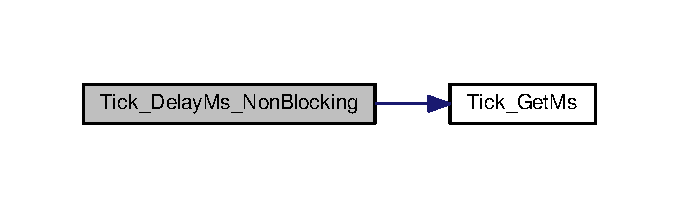
\includegraphics[width=326pt]{tick_8c_a700a086c5fb6a2a2491026af0fda77a8_cgraph}
\end{center}
\end{figure}


\hypertarget{tick_8c_a5018c28a90fe9864e870a712c8e2b571}{\index{tick.\+c@{tick.\+c}!Tick\+\_\+\+Get\+Ms@{Tick\+\_\+\+Get\+Ms}}
\index{Tick\+\_\+\+Get\+Ms@{Tick\+\_\+\+Get\+Ms}!tick.\+c@{tick.\+c}}
\subsubsection[{Tick\+\_\+\+Get\+Ms}]{\setlength{\rightskip}{0pt plus 5cm}uint32\+\_\+t Tick\+\_\+\+Get\+Ms (
\begin{DoxyParamCaption}
\item[{void}]{}
\end{DoxyParamCaption}
)}}\label{tick_8c_a5018c28a90fe9864e870a712c8e2b571}


return the number of mili-\/seconds since power up. 

\begin{DoxyReturn}{Returns}
number of mili-\/seconds.
\end{DoxyReturn}
\begin{DoxyNote}{Note}
the tick counter is expected to overflow and therefore code using the tick value should take this into account. 
\end{DoxyNote}


Here is the caller graph for this function\+:\nopagebreak
\begin{figure}[H]
\begin{center}
\leavevmode
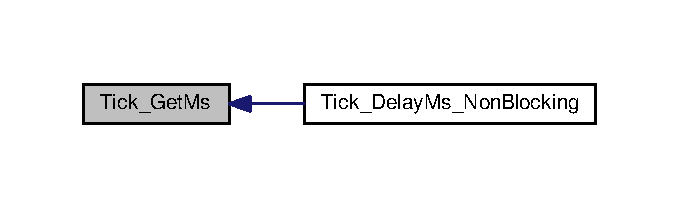
\includegraphics[width=326pt]{tick_8c_a5018c28a90fe9864e870a712c8e2b571_icgraph}
\end{center}
\end{figure}



\hypertarget{usart2_8c}{\section{/home/vagrant/\+Workspaces/\+Embedded/\+U\+S\+A\+R\+T/usart/src/\+M\+C\+U/usart2.c File Reference}
\label{usart2_8c}\index{/home/vagrant/\+Workspaces/\+Embedded/\+U\+S\+A\+R\+T/usart/src/\+M\+C\+U/usart2.\+c@{/home/vagrant/\+Workspaces/\+Embedded/\+U\+S\+A\+R\+T/usart/src/\+M\+C\+U/usart2.\+c}}
}


S\+T\+M32 serial2 M\+C\+U hardware interface layer. to maintain code portability, the hardware related code is split from the main logic.  


{\ttfamily \#include \char`\"{}M\+C\+U/usart2.\+h\char`\"{}}\\*
Include dependency graph for usart2.\+c\+:\nopagebreak
\begin{figure}[H]
\begin{center}
\leavevmode
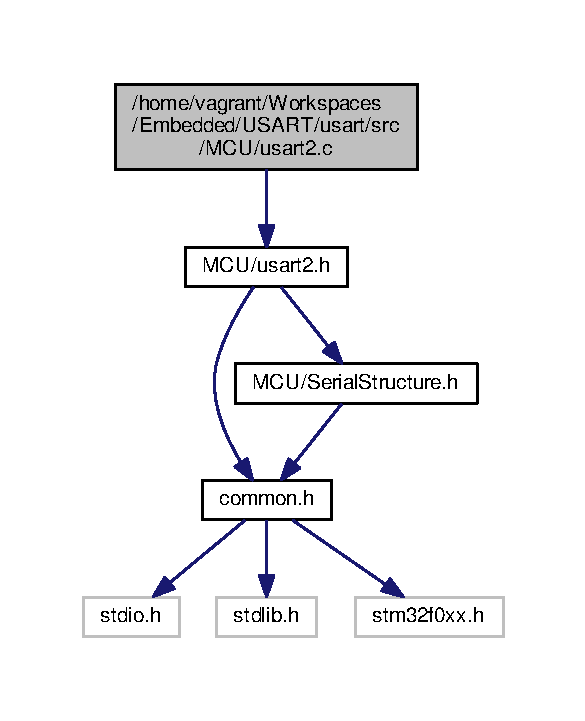
\includegraphics[width=281pt]{usart2_8c__incl}
\end{center}
\end{figure}
\subsection*{Macros}
\begin{DoxyCompactItemize}
\item 
\hypertarget{usart2_8c_a7bc0edf283b01a071b7ed8451eada11c}{\#define \hyperlink{usart2_8c_a7bc0edf283b01a071b7ed8451eada11c}{G\+P\+I\+O\+\_\+\+A\+F\+R\+L\+\_\+\+A\+F\+R2\+\_\+0}~(uint32\+\_\+t) 0x00000100}\label{usart2_8c_a7bc0edf283b01a071b7ed8451eada11c}

\begin{DoxyCompactList}\small\item\em Alternative function set bit 1 for A\+F\+R2. \end{DoxyCompactList}\item 
\hypertarget{usart2_8c_af91c2a8b8c966e16328c4384d1a31b23}{\#define \hyperlink{usart2_8c_af91c2a8b8c966e16328c4384d1a31b23}{G\+P\+I\+O\+\_\+\+A\+F\+R\+L\+\_\+\+A\+F\+R3\+\_\+0}~(uint32\+\_\+t) 0x00001000}\label{usart2_8c_af91c2a8b8c966e16328c4384d1a31b23}

\begin{DoxyCompactList}\small\item\em Alternative function set bit 1 for A\+F\+R3. \end{DoxyCompactList}\end{DoxyCompactItemize}
\subsection*{Variables}
\begin{DoxyCompactItemize}
\item 
\hyperlink{struct_serial_interface}{Serial\+Interface} \hyperlink{usart2_8c_a0ad9cd4fbffc7497abd537641dcc99af}{Serial\+Port2}
\begin{DoxyCompactList}\small\item\em Defines the standard serial functions for usart 2. \end{DoxyCompactList}\end{DoxyCompactItemize}


\subsection{Detailed Description}
S\+T\+M32 serial2 M\+C\+U hardware interface layer. to maintain code portability, the hardware related code is split from the main logic. 

\begin{DoxyAuthor}{Author}
\+: Ronald Sousa (Opticalworm) 
\end{DoxyAuthor}


\subsection{Variable Documentation}
\hypertarget{usart2_8c_a0ad9cd4fbffc7497abd537641dcc99af}{\index{usart2.\+c@{usart2.\+c}!Serial\+Port2@{Serial\+Port2}}
\index{Serial\+Port2@{Serial\+Port2}!usart2.\+c@{usart2.\+c}}
\subsubsection[{Serial\+Port2}]{\setlength{\rightskip}{0pt plus 5cm}{\bf Serial\+Interface} Serial\+Port2}}\label{usart2_8c_a0ad9cd4fbffc7497abd537641dcc99af}
{\bfseries Initial value\+:}
\begin{DoxyCode}
= \{
                                    IsSerialOpen,
                                    Open,
                                    Close,
                                    SendByte,
                                    SendString,
                                    SendArray,
                                    DoesReceiveBufferHaveData,
                                    GetByte
                                \}
\end{DoxyCode}


Defines the standard serial functions for usart 2. 

\begin{DoxySeeAlso}{See also}
\hyperlink{struct_serial_interface}{Serial\+Interface} 
\end{DoxySeeAlso}

%--- End generated contents ---

% Index
\newpage
\phantomsection
\addcontentsline{toc}{chapter}{Index}
\printindex

\end{document}
